% !TeX program = xelatex
\documentclass[a4paper,14pt]{extarticle} % Использование extarticle для 14pt шрифта
\usepackage{fontspec} % Для использования системных шрифтов	
\usepackage{polyglossia} % Для многоязыковой поддержки
\usepackage{amsmath}
\usepackage{amsfonts}
\usepackage{amssymb}
\usepackage{listings}
\usepackage{xcolor}
\usepackage{indentfirst} % Для отступа в первом абзаце
\setlength{\parindent}{1.25cm} % Установка отступа в 1.25 см
\setlength{\parskip}{0em} % Установка межабзацного интервала в 0

\newfontfamily\cyrillicfonttt{Courier New}

\lstset{ 
    language=[Sharp]C,              % Язык кода - C#
    basicstyle=\ttfamily\footnotesize, % Основной стиль шрифта
    keywordstyle=\color{blue},       % Цвет ключевых слов
    commentstyle=\color{green},      % Цвет комментариев
    stringstyle=\color{red},         % Цвет строк
    numbers=left,                   % Номера строк слева
    numberstyle=\tiny\color{gray},  % Стиль номеров строк
    stepnumber=1,                   % Нумерация каждой строки
    numbersep=5pt,                  % Расстояние между номерами строк и кодом
    showspaces=false,               % Показывать пробелы
    showstringspaces=false,         % Показывать пробелы внутри строк
    showtabs=false,                 % Показывать табуляцию
    frame=single,                   % Рамка вокруг кода
    tabsize=4,                      % Размер табуляции
    captionpos=b,                   % Позиция заголовка (b - снизу)
    breaklines=true,                % Перенос строк
    breakatwhitespace=false,        % Переносить строки только на пробелах
    title=\lstname,                 % Показывать название файла
    escapeinside={\%*}{*)},         % ЛаТеХ команды внутри кода
    morekeywords={var, get, set}    % Дополнительные ключевые слова
}

\renewcommand{\lstlistingname}{Лістинг} % Зміна підпису лістингу на українську мову

\setmainlanguage{ukrainian} % Основной язык документа
\setotherlanguage{english} % Дополнительный язык документа
\setmainfont{Times New Roman} % Установка шрифта Times New Roman
\usepackage{geometry} % Пакет для настройки полей страницы
\geometry{
    left=3cm,
    right=1.5cm,
    top=2cm,
    bottom=2cm
}

\usepackage{titlesec} % Пакет для настройки заголовков
\titleformat{\section}{\large\bfseries}{\thesection}{1em}{}
\titleformat{\subsection}{\normalsize\bfseries}{\thesubsection}{1em}{}

\usepackage{setspace} % Пакет для настройки межстрочного интервала
\onehalfspacing % Установка полуторного интервала

\usepackage{tocloft} % Пакет для настройки оглавления
\renewcommand{\cftsecleader}{\cftdotfill{\cftdotsep}} % Добавление точек к оглавлению

\usepackage{fancyhdr} % Пакет для настройки колонтитулов
\pagestyle{fancy}
\fancyhf{}
\fancyfoot[C]{\thepage}
\renewcommand{\headrulewidth}{0pt} % Убирает линию вверху страницы
\renewcommand{\footrulewidth}{0pt} % Убирает линию внизу страницы

\usepackage{graphicx}
\usepackage{caption} % Пакет для підписів до зображень
\usepackage{hyperref} % Пакет для создания кликабельных ссылок
\usepackage{float}
\usepackage{tabularx}
\usepackage{longtable}

\begin{document}	

    % Титульная страница
	\begin{titlepage}
		\centering
		\normalsize
		Київський національний університет імені Тараса Шевченка\\
		Факультет комп’ютерних наук та кібернетики\\
		Кафедра математичної інформатики\\
		
		\vspace*{4cm}
		
		\Large Курсова робота на тему: \\
		\textbf{Розробка методики порівняння ефективності алгоритмів патерн-метчингу}
		
		\vspace{2cm}
		
		\normalsize
			\begin{tabbing}
			\hspace{11cm} \= \hspace{5cm} \kill
			Виконав студент 3-го курсу \> \\ 
			Гришечкін Тихон Сергійович \> \underline{\makebox[5cm]{}}\\
			\> \makebox[5cm][c]{підпис} \\
			\\
			Науковий керівник: \> \\ 
			доцент, доктор фізико-математичних наук \> \\
			Завадський Ігор Олександрович \> \underline{\makebox[5cm]{}}\\
			\> \makebox[5cm][c]{підпис} \\
		\end{tabbing}
		
		\vfill
		
		\begin{flushright}
			\normalsize
			Засвідчую, що в цій курсовій роботі немає запозичень \\
			з праць інших авторів без відповідних посилань.\\
			\vspace{1em} % Пропуск одного рядка
			\hspace*{0em}Студент \hspace{1cm} \underline{\makebox[5cm]{}}\\
			\makebox[5cm][c]{підпис}
		\end{flushright}
		
		
		\vfill
		
		\centering
		\normalsize
		Київ, 2024
		
	\end{titlepage}

	
	\newpage

	\section*{Реферат}

	Обсяг роботи 29 сторінок, 7 ілюстрацій, 24 таблиці, 7 джерел посилань.

	АЛГОРИТМИ. ПОШУК, РЯДКИ, ПАТЕРН,
	ЕФЕКТИВНІСТЬ, ОЦІНКИ, ШАБЛОН, ТЕСТУВАННЯ, МЕТЧИНГ

	Об'єктом роботи є аналіз та порівняння єфективності алгоритмів патерн-метчингу.
	
	Предметом роботи є розробка методики порівняння ефективності алгоритмів патерн-метчингу.

	Метою роботи є порівняння ефективності алгоритмів патерн-метчингу на практиці. 

	Інструменти розробки: операційна система - Windows 10. Середовище розробки - \textit{Clion} та \textit{Pycharm} для візуалізації результатів.

	Результати роботи : виконано загальний огляд проблеми, розглянуто та описано існуючі алгоритми патерн-метчингу.
	Розроблена методика порівняння ефективності алгоритмів патерн-метчингу. Виконано порівняння ефективності набору алгоритмів на практиці.
	Продемонстровано результати порівняння та зроблено відповідні висновки.

	Робота може бути корисна для вибору оптимального алгоритму патерн-метчингу та ознайомлення з темою алгоритмів патерн-метчингу.

	Також запропоновані можливі розвинення та нові дослідження за заданою тематикою.

	\newpage

    % Оглавление
    \tableofcontents


    \newpage
    
    % Вступ
    \section*{Вступ}
	\addcontentsline{toc}{section}{Вступ}

	\textbf{Оцінка сучасного стану об’єкта дослідження:}
	
	Задача патерн-метчингу є дуже важливою задачею в інформатиці. Вона має широке застосування в ЇЇ різних областях, зокрема:
\begin{itemize}
    \item Інформаційний пошук: Алгоритми пошуку використовуються в пошукових системах для
	знаходження релевантних документів на основі запитів користувачів.
    \item Біоінформатика: Пошук рядків є ключовим у знаходженні послідовностей нуклеотидів або амінокислот у геномах та протеомах. \cite{dna}
    \item Обробка текстів: Алгоритми пошуку використовуються для знаходження та заміни текстових фрагментів у текстових редакторах.
    \item Бази даних: Пошук рядків використовується в базах даних для виконання запитів зі згадками текстових фрагментів або шаблонів.
    \item Компіляція: Компілятори використовують алгоритми пошуку підрядків для аналізу та оптимізації програмного коду.

\end{itemize}


\textbf{Актуальність роботи та підстави для її виконання:}

Потреба у використанні алгоритмів пошуку на практиці зростає. Кожного року з'являється і пропонується все більше алгоритмів патерн-метчингу. А отже розробка методики порівняння цих алгоритмів, є важливим напрямом роботи.

Існує декілька досліджень з порівняння алгоритмів патерн метчингу (\cite{smart}, \cite{exact}, \cite{experiment}). У всіх з них використовується схожа методика оцінки ефективності алгоритмів.
У цій роботі я пропоную і обгрунтовую нову власну методику порівняння ефективності алгоритмів.

\textbf{Мета роботи:} Розробка методики порівняння ефективності алгоритмів патерн метчингу.

\textbf{Завдання:} Порівняти ефективності алгоритмів патерн-метчингу за створеною методикою.

\textbf{Засоби дослідження та розробки:}

Використовувалось середовище розробки \textit{Clion} для мови програмування \textit{c++}, де було розроблену програму для тестування алгоритмів пошуку. Також було використано середовище розробки \textit{Pycharm} для візуалізації отриманих результатів.

\textbf{Можливі сфери застосування:}

Дана курсова робота може допомогти при виборі оптимального алгоритму патерн-метчингу для своєї задачі. За допомогою цієї роботи можна ознайомитись з методами алгоритмів пошуку рядка, їх класифікацією, ефективністю та іншою корисною інформацією по цій темі.
Також робота може бути корисною для розробки власних методів порівняння ефективності алгоритмів. 

    \newpage



    % Основна частина
    \section{Алгоритми пошуку рядка}

	\subsection{Постановка задачі патерн-метчингу}

	Нехай дані дві послідовності: текст \( T \) та патерн \( P \) (далі також інколи позначається, як <<шаблон>>), де \( |T| = n \) та \( |P| = m \). Задача полягає у знаходженні всіх входжень патерна \( P \) у текст \( T \).

При цьому передбачається, що:
\begin{itemize}
    \item \( T \) та \( P \) складаються з символів алфавіту \( \Sigma \).
    \item Алфавіт \( \Sigma \) може бути скінченним або нескінченним, але у нашій постановці розглядається скінченний алфавіт.
\end{itemize}


Розглядається задача пошуку підстроки у формулюванні \textbf{single-pattern matching}, що передбачає пошук одного заданого патерна в тексті. Не розглядаються задачі \textbf{approximate pattern searching}, де потрібно знаходити патерни з певною степенню схожості, або \textbf{regular pattern searching}, де патерн може бути виражений у вигляді регулярного виразу.


	\subsection{Загальна характеристика алгоритмів пошуку рядка}

	Найпростішим методом для пошуку підрядка в рядку є алгоритм повного перебору (brute force). Його суть полягає у перевірці кожної позиції в тексті \( T \) як можливої початкової позиції для патерна \( P \). Для кожної такої позиції перевіряється, чи співпадає патерн \( P \) з відповідною підстрокою в тексті \( T \). Цей метод має часову складність \( O(n \cdot m) \), де \( n \) – довжина тексту, а \( m \) – довжина патерна. Через високу обчислювальну складність цей алгоритм є дуже неоптимальним для великих текстів і патернів.

	У 1970 році Д. Морріс та В. Пратт \cite{morris-pratt} розробили перший оптимальний алгоритм пошуку підстроки – алгоритм Кнута-Морріса-Пратта (KMP). Цей алгоритм значно покращив ефективність пошуку, зменшивши часову складність до \( O(n + m) \).

	З часом з'явилося багато інших алгоритмів (більше 124 див. \cite{smart}). Всі ці алгоритми можна умовно поділити на чотири основні категорії:
	\begin{itemize}
		\item алгоритми на основі порівняння символів
		\item  алгоритми на основі суфіксних автоматів
		\item алгоритми на основі побітового паралелізму
		\item гібридні алгоритми.
	\end{itemize}

\textbf{Алгоритми на основі порівняння символів}

Алгоритми на основі порівняння символів (character-based approaches або comparison based approaches) є класичним підходом, який просто порівнює символи для вирішення задач пошуку рядка.

Алгоритми на основі порівняння символів мають дві основні стадії: пошук і зсув. Алгоритм Бойера-Мура \cite{bm}, є стандартним та еталонним методом цього типу. Він використовує таблицю зсувів для пропуску непотрібних порівнянь, що значно підвищує швидкість пошуку.

\textbf{Алгоритми на основі суфіксних автоматів}

Суфіксний автомат (Suffix automaton) складається з детермінованого ациклічного кінцевого автомата, що приймає всі суфікси заданого рядка.

Ці алгоритми спочатку будують суфіксний автомат заданого патерна, а потім використовують його для знаходження входжень патерна в текст.
Прикладом алгоритму даного класу є є Backward-DAWG-Matching алгоритм (BDM).

\textbf{Алгоритми на основі побітового паралелізму}

Алгоритми на основі паралелізму бітового рівня були запропоновані для прискорення процесу пошуку шляхом використання внутрішнього паралелізму бітових операцій, що зменшує кількість операцій у рази до $\omega$, де $\omega$ –  кількость бітів у машинному слові.

Ці алгоритми є швидкими та ефективними, особливо коли довжина патерна менша за довжину машинного слова. До таких алгоритмів належать наприклад Shift-OR (SO), Shift-AND (SA) алгоритми.

\textbf{Гібридні алгоритми}

Гібридні алгоритми комбінують переваги різних методів для вирішення складних задач. Вони поєднують методи з різних категорій для досягнення кращої ефективності.

Таким чином, за роки розвитку цієї області задач з'явилося багато алгоритмів для пошуку підрядка, які можна класифікувати за чотирма основними категоріями. Кожен клас алгоритмів має свої недоліки та переваги, які важливо розуміти при виборі оптимального алгоритму для своєї задачі.

\subsection{Алгоритм Бойера-Мура}
Розглянемо детальніше деякі алгоритми пошуку.

Першим розглянемо алгоритм Бойера-Мура (BM), який є класичним представником класу <<character-based>> алгоритмів.

Алгоритм шукає входження патерну $\textbf{p}$, прикладаючи його до тексту $\textbf{t}$ зліва направо, але при цьому порівняння, виконуються справа наліво, починаючи з останнього символу патерну.

Далі якщо при порівнянні знайдено перший неспівпадаючий символ патерну, то виконується зсув патерну на деяку кількість позицій, за допомогою наступних евристик:

\begin{itemize}
	\item \textit{Евристика стоп символів}:
	
	Для цього для кожного символу алфавіту $\Sigma$ запам'ятовуємо індекс останнього його входження в патерн, якщо він є, або запам'ятовуємо -1, якщо він не входить в патерн (вважаємо, що індексація символів починається з нуля). 
	Назвемо цей масив індексів $StopTable$.
	
	Тепер розглянемо символ тексту $c$, що не співпав на поточній ітерації порівняння. Позначимо поточний індекс патерну на якому відбулось неспівпадіння як $i$.
	Тоді якщо виконується \[i-StopTable[c] > 0\] то відбувається зсув патерну на $i-StopTable[c]$ кроків, інакше кажучи на найменшу кількість кроків щоб відбулось співпадіння з символом $c$. (рис. \ref{fig:boyer_moore})
	\item \textit{Евристика співпадаючого суфікса}:
	
	Якщо при порівнянні шаблону справа наліво збігся суфікс \( S \), а символ \( c \), що стоїть перед \( S \) в шаблоні не збігся (тобто шаблон має вигляд \( PcS \)),
 	то евристика співпадаючого суфікса зсуває шаблон на найменше число позицій вправо так, щоб рядок \( S \) збігся з шаблоном, а символ, що передує даному збігу \( S \) в шаблоні, відрізнявся б від \( c \).
	
	Заради цього для патерну $p$ перед початком пошуку, обраховуються відповідні величини зсуву, за допомогою алгоритму,
	схожого за ідеєю на алгоритми обчислення <<префікс-функції>> та <<Z-функції>>.

	Як і випадку цих алгоритмів ці зсуви обчислюються за $O(m)$ операцій.
	
	Далі в алгоритмі просто використовуються ці заздалегідь обчислені зсуви при неспівпадінні символів.

	Зазначимо, що якщо на кожній ітерації просто знову порівнювати символи, навіть з використанням зсувів асимптотика алгоритму
	складає $O(n*m)$ операцій. Для досягнення складності $O(n+m)$, треба не порівнювати з шаблоном вже співпадаючий суфікс, знайдений на попередній ітерації.

\end{itemize}
	\begin{figure}[H] % Починаємо середовище figure
		\centering % Центруємо малюнок
		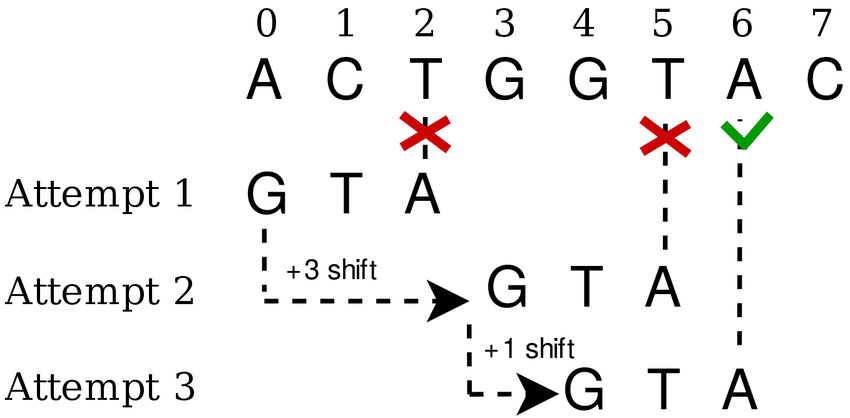
\includegraphics[width=0.6\textwidth]{images/boyer_moore.png} % Вставляємо малюнок
		\caption{Приклад використання евристики стоп символів} % Підпис до малюнка
		\label{fig:boyer_moore} % Мітка для посилань на малюнок
	\end{figure}
	\begin{figure}[H] % Починаємо середовище figure
		\centering % Центруємо малюнок
		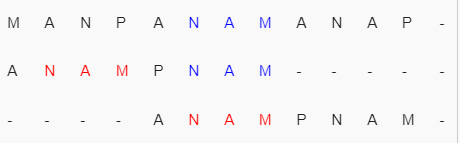
\includegraphics[width=0.6\textwidth]{images/boyer_moore_suffix.png} % Вставляємо малюнок
		\caption{Приклад використання евристики співпадаючого суфікса} % Підпис до малюнка
		\label{fig:boyer_moore_suffix} % Мітка для посилань на малюнок
	\end{figure}

    \newpage
	Додамо також, що існує багато модифікацій алгоритму Бойера-Мура, які використовують інші евристики або реалізують вже існуючі інакше.
	
	Прикладами таких алгоритмів є алгоритми Бойєра - Мура - Хорспула (BMH), Чжу - Такаокі (ZT), турбо - Бойера - Мура (TBM).

	Наприклад BMH використвує тільки <<евристику стоп символів>>, але тільки за останнім символом, тому є спрощени варіантом Бойера-Мура.

	ZT використовує також <<евристику стоп символів>>, але для пар символів, заради оптимізації при маленьких алфавітах.

	Зазначимо також, що довгі патерни зазвичай дають довші зсуви, тому алгоритми класу <<порівняння символів>> добре працюють на таких патернах.
	\subsection{Алгоритми Shift-OR (SO) та Shift-AND (SA)}

	Розглянемо алгоритми Shift-OR (SO) та Shift-AND (SA), які є представниками класу алгоритмів основаних на паралелізмі бітових операцій.

	Опишемо SA алгоритм.

	Нехай маємо $i$-й символ тексту $t$. 

	Введемо матрицю $Mask$ (рис \ref{fig:shift_or}), де
	\[Mask[i][j] = 1,\text{якщо } t[i-j..i] = p[0..j]\]
	\[Mask[i][j] = 0,\text{якщо } t[i-j..i] \neq  p[0..j]\]

	Тоді маємо входження шаблону на $i$-му кроці, коли $Mask[i][m-1] = 1$.
	\begin{figure}[H]
		\centering
		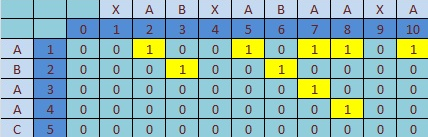
\includegraphics[width=0.6\textwidth]{images/sa_example.png}
		\caption{Приклад матриці $Mask$}
		\label{fig:shift_or}
	\end{figure}

	Але вичислення матриці $Mask$, на кожному кроці займає $O(m)$ операцій тому такий алгоритм нічим не краще <<Brute-Force>> алгоритму, і фактично ним і є.

	Тоді нехай маємо матрицю $pos$, де для символу $c$ маємо
	\[pos[c][j] = 1,\text{якщо } p[j]=c\]
	\[pos[c][j] = 0,\text{якщо } p[j] \neq c\]
	Можемо помітити наступну властивість. 
	$$Mask[i]=(Mask[i-1]<<1)\And pos[t[i]]$$

	Де $<<$ - операція побітового зсуву вліво.

	Тепер можемо в рамках реалізації замінити вектори $Mask[i]$ та $pos[c]$, на звичайні змінні, для яких всі операції будуть виконані $O(1)$, але отримаємо очевидне обмеження $m<\omega$, де $\omega$ - довжина машинного слова.

	Shift-or алгоритм аналогічний алгоритму Shift-and, де просто інвертовано вектори $Mask[i]$ та $pos[c]$, а операція $and$ замінюється на $or$. 
	А критерієм входження стає $Mask[i][m-1]=0$.

	Алгоритми, що основані на паралелізмі бітових операцій називаються так бо на кожному кроці виконується $\omega$ паралельних порівнянь, хоча фактично виконується лише декілька бітових операцій.

	Такі алгоритми дають значне прискорення на патернах невеликої довжини, для яких вони і були створені. Для $m>\omega$, зазвичай ці алгоритми оптимізують або об'єднують з іншими.

	Наприклад у SA, для патернів більшої довжини, при знаходженні співпадіння довжини $\omega$ решту символів просто перевіряють до першого неспівпадіння.

	Також перевагою цих алгоритмів є те, що вони легко модифікуються до <<наближеного пошуку входження рядка>> (approximate pattern searching).
	Ці алгоритми вбудовані у реалізацію Unix утиліти \textit{agrep}, що і виконує цей наближений пошук.
    
	\subsection{Алгоритм Forward Dawg Matching}
Розглянемо також алгоритм Forward Dawg Matching (FDM \cite{FDM}), що є представником класу <<automata-based>> алгоритмів.

Алгоритм Forward Dawg Matching обчислює найдовший підрядок шаблону, що закінчується на кожній позиції в тексті.

Це можливо завдяки використанню найменшого суфіксного автомата (також називається DAWG, Directed Acyclic Word Graph) для шаблону. Найменший суфіксний автомат слова \( w \) - це детермінований кінцевий автомат \( S(w) = (Q, q_0, T, E) \). Мова, прийнята \( S(w) \), це \( L(S(w)) = \{u \in \Sigma^* : \exists v \in \Sigma^* \text{ така, що } w = vu\} \).

Підготовча фаза алгоритму Forward Dawg Matching полягає в обчисленні найменшого суфіксного автомата для шаблону \( x \). Це займає лінійний час та простір додаткової пам'яті відносно довжини шаблону.

Під час фази пошуку алгоритм Forward Dawg Matching аналізує символи тексту зліва направо за допомогою автомата \( S(x) \), починаючи з початкового стану \( q_0 \). Для кожного стану \( q \) у \( S(x) \) найдовший шлях від \( q_0 \) до \( q \) позначається як \( \text{length}(q) \).

Структура автомата використовує поняття суфіксних посилань. Для кожного стану \( q \) суфіксне посилання \( q \) позначається як \( S[q] \).

S[q] - посилання на стан автомата, що є найбільшим суфіксом стану q.

\begin{figure}[H]
	\centering
	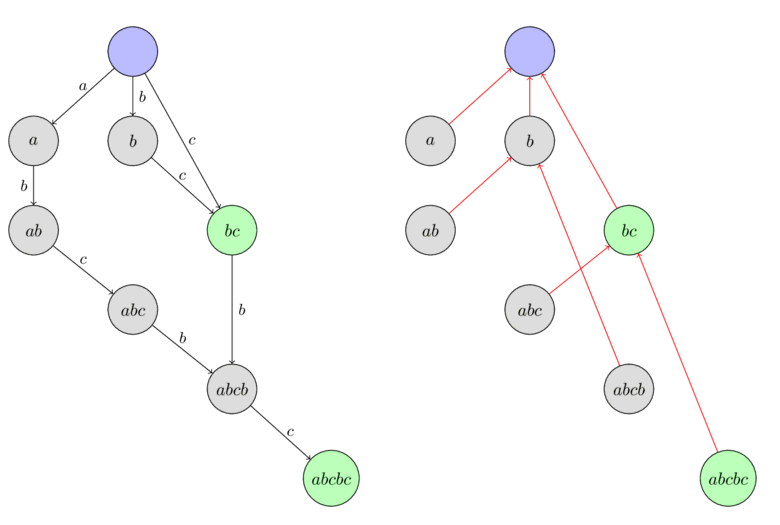
\includegraphics[width=0.6\textwidth]{images/suffix_automata.png}
	\caption{Приклад суфіксного автомата рядка "abcbc", з його суфіксними посиланнями}
	\label{fig:fdm}
\end{figure}

Для стану \( p \) нехай \( \text{Path}(p) = (p_0, p_1, \ldots, p_{\ell}) \) буде суфіксним шляхом \( p \), таким чином що \( p_0 = p \), для \( 1 \leq i \leq \ell \), \( p_i = S[p_{i-1}] \) і \( p_{\ell} = q_0 \).

Для кожного символу тексту \( t[j] \) послідовно, нехай \( p \) буде поточним станом, тоді алгоритм Forward Dawg Matching здійснює перехід, по символу \( t[j] \) для першого стану \( \text{Path}(p) \), для якого такий перехід визначений. Поточний стан \( p \) оновлюється за допомогою цільового стану цього переходу або початкового стану \( q_0 \), якщо не існує переходу по символу \( t[j] \) з будь-якого стану \( \text{Path}(p) \).

Збіг шаблону \( x \) знайдено, коли \( \text{length}(p) = m \), де $m =|x|$.

Недоліками алгоритмів, що основані на суфіксних автоматах є додаткові витрати на побудову автомата.

Перевагами таких алгоритмів є те що, їх можна реалізувати так, щоб співпадіння на кожному новому індексі тексту було знайдено  простими переходами по автомату, за $O(1)$ операцій, що підходить для так званих <<real-time-systems>>.

Також перевагою є те, що на кожному кроці алгоритм знаходить найбільший підрядок шаблону, що закінчується на поточній позиції тексту, а отже вирішує більш загальну задачу ніж пошук входжень патерна в текст.
% Практична частина
	\newpage
    \section{Порівняння ефективності алгоритмів}

	\subsection{Фактори впливу на ефективність алгоритмів}

	Одразу зазначимо, що не будемо порівнювати алгоритми за об'ємом зайнятої додаткової пам'яті, адже більшість алгоритмів займають $O(m)$, або $O(m*|\Sigma|)$ додаткової пам'яті, що є незначним показником при невеликих патернах та алфавітах на яких в більшості випадків виконують пошук.
	
	Також зазначимо, що в цій роботі не будуть порівнюватись алгоритми, що виконують препроцесинг над текстом (так звані <<offline exact string matching algorithms>>), адже їх потрібно порівнювати окремо від <<онлайн>> алгоритмів.

	Наведемо основні фактори впливу на швидкодію алгоритмів патерн метчингу:
	\begin{itemize}
		\item $|T|$ - довжина тексту.
		\item $|P|$ - довжина шаблону.
		\item $|\Sigma|$ - розмір алфавіту.
		\item Кількість різних підрядків $P$ та $T$.
		\item Кількість входжень $P$ в $T$.
		\item Граматика мови, до якої належить текст і шаблон (якщо існує).
		\item "Ворожість" користувача. Іншими словами: чи буде користувач навмисно задавати дані, на яких алгоритм повільно працюватиме?
		\item Архітектура процесора. Деякі процесори мають автоінкрементні або SIMD-операції, які дозволяють швидко порівняти дві ділянки ОЗП (наприклад, rep cmpsd x86). Деякі алгоритми використовують такі операції (SSE Filter Algorithm).
		\item Характер даних шаблона $P$ у порівнянні з $T$. Наприклад якщо $P$ - деяке число, що шукається в англійському тексті, то більшість $character-based$ алгоритмів оптимізує пошук використовуючи свої евристики зсуву. 
	\end{itemize}

	Додамо що цей перелік не є кінцевим і можна навести ще багато інших факторів впливу.

	\subsection{Методика порівняння алгоритмів}\label{methodic}

	У праці Ф. Саймона та Л. Тьєррі \cite{experiment} та інших роботах з порівнянням алгоритмів патерн-метчингу, при порівнянні алгоритмів пошуку, увагу було зосереджено на великій кількості алгоритмів та різних можливих вхідних текстах.
	При тестуванні патерни завжди обирались випадковим чином із тексту.

	Тому у власній роботі, я вирішив розширити множину можливих патернів і порівняння будуть виконуватись по наступним типам патернів:
	\begin{itemize}
		\item Випадкові патерни, заданого алфавіту.
		\item Патерни випадковим чином, обрані із заданого тексту.
		\item Патерни, що часто зустрічаються в тексті. Наприклад для тексту англійської літератури було обрано патерни найбільш повторюваних слів англійської мови. Аналогічно для української - найбільш повторюваних слів української мови. Для json бази даних - деякі ключові слова та значення полів, що часто зустрічаються.
	\end {itemize}

	Також зазначу, що не було спроби визначити ефективність алгоритмів, за рядом експериментів, окрім як просумувати абсолютні значення часу виконання алгоритмів.

	Тому у власній роботі я вводжу поняття відносного результату роботи алгоритму $\sigma_{\text{алг}}$.

	Нехай ми порівнюємо деяку множину алгоритмів. Нехай деякий алгоритм на тесті відпрацював найшвидше з усіх за час $t_{\text{min}}$.

	Тоді відносний результат алгоритму, що відпрацював за час $t_{\text{алг}}$, дорівнює:
	$$\sigma_{\text{алг}} = \frac{t_{\text{алг}}-t_{\text{min}}}{t_{\text{min}}}$$
    
	Відносний результат показує у скільки разів алгоритм відхилився від оптимального на тесті. Абсолютним результатом будемо називати $t_{\text{алг}}$.
	
	Сумарним середнім відносним результатом будемо називати середнє арифметичне відносних результатів алгоритма на деякій кількості тестів.
	
	Введення відносних результатів дозволяє зробити загальний аналіз результатів роботи алгоритмів за декількома експериментами.

	Наприклад маємо такі результати роботи алгоритмів (табл \ref{table:times}):
	\begin{table}[H]
		\centering
		\begin{tabular}{|c|c|c|}
			\hline
			& \textbf{Алгоритм 1} & \textbf{Алгоритм 2} \\ 
			\hline
			\textbf{Тест 1} & 40 & 20 \\ 
			\hline
			\textbf{Тест 2} & 500 & 700 \\ 
			\hline
		\end{tabular}
		\caption{Абсолютні результати алгоритмів у мс}
		\label{table:times}
	\end{table}

	Тоді маємо наступні відносні результати роботи алгоритмів (табл \ref{table:relative_times}):
	\begin{table}[H]
		\centering
		\begin{tabular}{|c|c|c|}
			\hline
			& \textbf{Алгоритм 1} & \textbf{Алгоритм 2} \\ 
			\hline
			\textbf{Тест 1} & 1 & 0 \\ 
			\hline
			\textbf{Тест 2} & 0 & 0.4 \\ 
			\hline
		\end{tabular}
		\caption{Відносні результати алгоритмів $\sigma$}
		\label{table:relative_times}
	\end{table}

	Сумарний час виконання 1 алгоритму - 540 мс. Сумарний середній відносний результат $(1+0)/2=0.5$.

	Сумарний час виконання 2 алгоритму - 720 мс. Сумарний середній відносний результат $(0+0.4)/2=0.2$.

	Маємо що 1-й алгоритм сумарно працював менше часу, а 2-й в середньому менше відхилявся від оптимального за тестом.

	Середній відносний результат може бути непоганою оцінкою роботи алгоритма за декількома тестами, хоча можливо можна обрати більш доцільну формулу для обчислення $\sigma_{\text{алг}}$.

	Далі я буду користуватись формулою наданою в цьому підрозділі.

	Додамо що в практичній частині для порівняння, тести будуть проводитися на наступних текстах:

	\begin{itemize}
		\item Англійська література - <<The Lord of the Rings: The Fellowship of the Ring>>
		\item Українська література - <<Лісова пісня>>
		\item Випадкова послідовність геному.
		\item Json база даних.
		\item Велика веб сторінка (html).
		\item rand2 - випадковий рядок на алфавіті довжини 2
		\item rand32 - випадковий рядок на алфавіті довжини 32
		\item rand64 - випадковий рядок на алфавіті довжини 64
		\item Великий текст на мові програмування $c$.
	\end{itemize}
	\subsection{Набір алгоритмів для порівняння} \label{section:algorithms_set}

	Для порівняння ефективності алгоритмів на практиці мною було обрано наступні алгоритми (табл \ref{table:string_algorithms}):

	\begin{table}[H]
		\centering
		\small
		\begin{tabular}{|c|c|c|c|}
			\hline
			& \textbf{Повна назва} & \textbf{Рік розробки} & \textbf{Клас алгоритму} \\ 
			\hline
			\textbf{KR} & Karp-Rabin & 1987 & comparison \\ 
			\hline
			\textbf{KMP} & Knuth-Morris-Pratt & 1977 & comparison \\ 
			\hline
			\textbf{BNDMQ2} & BNDM with q-grams & 2009 & bit-parallelism \\ 
			\hline
			\textbf{BM} & Boyer-Moore & 1977 & comparison \\ 
			\hline
			\textbf{BXS} & BNDM with Extended Shifts &  2010 & bit-parallelism \\ 
			\hline
			\textbf{BOM} &  Backward-Oracle-Matching & 1999 & automata \\ 
			\hline
			\textbf{Skip} & Skip-Search  & 1998 & comparison \\ 
			\hline
			\textbf{Hash3} & Wu-Manber algorithm	 & 2007 & comparison \\ 
			\hline
			\textbf{FS} & Fast-Search &  2003 & comparison \\ 
			\hline
			\textbf{SSM} & Simple String Matching & 2015 & hybrid \\ 
			\hline
			\textbf{SBNDM} & Simplified BNDM & 2003 & bit-parallelism \\ 
			\hline
			\textbf{BSDM} & Backward SNR DAWGM & 2012 & automata \\ 
			\hline
		\end{tabular}
		\caption{Інформація про обрані алгоритми пошуку рядка}
		\label{table:string_algorithms}
	\end{table}

	При виборі набору алгоритмів орієнтувався на набір, що містиме деякі класичні алгоритми (\textbf{KR},\textbf{KMP},\textbf{BM}), для порівняння з сучасними. Інші обирались так, щоб алгоритмів різних класів було представлено приблизно порівну.

	
	\newpage
	\section{Практична частина}
	
	\subsection{Порівняння алгоритмів на випадкових патернах}
	В цьому підрозділі будемо порівнювати алгоритми на повністю випадкових патернах, заданого алфавіту для кожного тесту. 

	\textbf{Середовище тестування:}

	Всі тестування проводились на персональному комп'ютері з наступними характеристиками:
	\begin{itemize}
		\item \textbf{Процесор:} Intel(R) Core(TM) i7-9750H CPU 2.60GHz
		\item \textbf{Оперативна пам'ять:} 16.0 GB
		\item \textbf{Жорсткий диск:} 512 GB SSD
		\item \textbf{Операційна система:} Windows 10 Home 64-bit
		\item \textbf{Графічний процесор:} NVIDIA GeForce GTX 1650 8GB
	\end{itemize}

	Проведемо тестування на англійському тексті (<<The Lord of the Rings: The Fellowship of the Ring>>, табл. \ref{table:lotr}), та випадкових патернах довжини m. $$m=2^k, (1<=k<=12)$$
	Додамо що, результат вказаний у табл. \ref{table:lotr} обраховувався не одним тестуванням, а для кожного $m$ проводилась константна кількість (в моєму випадку 30) раундів тестування, і сумарний час їх виконання для кожного алгоритму було записано у таблицю.

	\begin{table}[H]
		\centering
		\scriptsize
		\begin{tabular}{|c|c|c|c|c|c|c|c|c|c|c|c|c|}
		\hline
		\textbf{m} & \textbf{KR} & \textbf{KMP} & \textbf{BNDMQ2} & \textbf{BM} & \textbf{BXS} & \textbf{BOM} & \textbf{Skip} & \textbf{Hash3} & \textbf{FS} & \textbf{SSM} & \textbf{SBNDM} & \textbf{BSDM} \\
		\hline
		2 & 148.09 & 232.28 & 157.14 & 187.87 & 60.26 & 225.18 & 57.41 & 232.22 & 154.28 & 138.43 & 198.38 & \textbf{49.66} \\
		\hline
		4 & 139.92 & 230.29 & 51.46 & 95.36 & 31.52 & 167.41 & 31.58 & 265.74 & 77.60 & 67.08 & 71.31 & \textbf{29.69} \\
		\hline
		8 & 129.49 & 226.57 & 22.05 & 46.34 & 14.96 & 136.70 & 15.57 & 90.37 & 38.90 & 33.42 & 30.36 & \textbf{13.64} \\
		\hline
		16 & 132.52 & 228.02 & 10.62 & 23.38 & 9.41 & 131.90 & 10.14 & 39.02 & 20.21 & 17.19 & 14.39 & \textbf{9.03} \\
		\hline
		32 & 135.19 & 226.09 & \textbf{5.97} & 12.66 & 6.36 & 125.83 & 7.05 & 18.99 & 11.07 & 9.46 & 7.47 & 7.23 \\
		\hline
		64 & 130.19 & 225.36 & 5.58 & 7.06 & \textbf{4.72} & 119.16 & 5.43 & 9.88 & 6.27 & 5.20 & 5.58 & 5.96 \\
		\hline
		128 & 134.70 & 225.72 & 5.46 & 4.60 & \textbf{3.64} & 93.22 & 4.97 & 5.97 & 4.37 & \textbf{3.64} & 5.63 & 6.00 \\
		\hline
		256 & 138.60 & 238.41 & 6.07 & 3.96 & 236.48 & 71.59 & 4.93 & 4.58 & 4.03 & \textbf{2.95} & 6.08 & 5.66 \\
		\hline
		512 & 130.37 & 223.59 & 5.47 & 3.63 & 225.89 & 46.16 & 4.74 & 4.26 & 3.71 & \textbf{2.73} & 6.29 & 5.64 \\
		\hline
		1024 & 134.62 & 227.50 & 5.93 & 3.69 & 226.83 & 41.15 & 5.86 & 4.01 & 4.09 & \textbf{3.03} & 6.33 & 6.09 \\
		\hline
		2048 & 129.63 & 228.63 & 5.53 & 3.89 & 228.88 & 54.92 & 7.95 & 4.23 & 4.43 & \textbf{3.61} & 5.83 & 6.18 \\
		\hline
		4096 & 135.46 & 229.16 & 5.76 & 5.36 & 229.06 & 104.23 & 14.62 & \textbf{5.27} & 5.99 & 5.51 & 6.95 & 6.77 \\
		\hline
		\end{tabular}
		\caption{Результати роботи алгоритмів на англійському тексті (час у мілісекундах)}
		\label{table:lotr}
		\end{table}

		Кожен найкращий результат за заданим $m$, виділено у таблиці жирним шрифтом. Зазначимо що результати тестуванням длі інших текстів, будуть виводитись аналогічним чином до табл. \ref{table:lotr} і протягом курсової роботи формат не змінюється.

		Проаналізуємо отримані результати. Бачимо, що SSM алгоритм отримує оптимальні результати на великих $m$, а BSDM та BXS - на невеликих.

		Бачимо що із класичних алгоритмів KR та KMP - показують дуже неоптимальні результати, а BM - результат близький до оптимального для великих $m$.

		Проведемо тестування на рядку rand32 (табл. \ref{table:rand32}).
		\begin{table}[H]
			\centering
			\scriptsize
			\begin{tabular}{|c|c|c|c|c|c|c|c|c|c|c|c|c|}
			\hline
			\textbf{m} & \textbf{KR} & \textbf{KMP} & \textbf{BNDMQ2} & \textbf{BM} & \textbf{BXS} & \textbf{BOM} & \textbf{Skip} & \textbf{Hash3} & \textbf{FS} & \textbf{SSM} & \textbf{SBNDM} & \textbf{BSDM} \\
			\hline
			2 & 13.50 & 22.25 & 14.80 & 18.45 & 5.96 & 21.28 & 5.39 & 22.51 & 15.75 & 13.21 & 19.45 & \textbf{4.82} \\
			\hline
			4 & 12.89 & 22.12 & 5.03 & 9.21 & 2.99 & 16.27 & 2.96 & 26.00 & 8.12 & 6.78 & 7.01 & \textbf{2.69} \\
			\hline
			8 & 13.57 & 22.80 & 2.24 & 4.66 & 1.77 & 13.72 & 1.85 & 8.88 & 4.44 & 3.46 & 3.78 & \textbf{1.57} \\
			\hline
			16 & 13.26 & 22.67 & 1.15 & 2.51 & 1.06 & 13.16 & 1.26 & 3.94 & 2.53 & 1.83 & 1.44 & \textbf{0.96} \\
			\hline
			32 & 12.92 & 22.41 & \textbf{0.61} & 1.25 & 0.67 & 12.10 & 0.76 & 1.89 & 1.54 & 0.96 & 0.78 & 0.79 \\
			\hline
			64 & 13.25 & 22.24 & 0.61 & 0.74 & \textbf{0.50} & 13.07 & 0.81 & 1.00 & 1.12 & 0.58 & 0.64 & 0.74 \\
			\hline
			128 & 13.93 & 22.53 & 0.55 & 0.50 & \textbf{0.36} & 11.54 & 0.83 & 0.62 & 0.92 & 0.45 & 0.69 & 1.06 \\
			\hline
			256 & 21.89 & 31.19 & 1.07 & \textbf{0.54} & 36.67 & 17.27 & 1.60 & 0.76 & 0.99 & 0.62 & 0.89 & 0.94 \\
			\hline
			512 & 19.64 & 27.87 & 0.85 & 1.50 & 30.04 & 17.61 & 1.86 & \textbf{0.44} & 1.13 & 0.71 & 1.56 & 0.92 \\
			\hline
			1024 & 13.42 & 22.32 & 0.54 & 0.79 & 22.37 & 22.14 & 2.89 & \textbf{0.48} & 1.26 & 1.05 & 0.63 & 0.99 \\
			\hline
			2048 & 13.47 & 23.30 & \textbf{0.58} & 1.49 & 23.01 & 46.59 & 6.12 & 0.70 & 1.92 & 1.98 & 0.64 & 1.46 \\
			\hline
			4096 & 13.00 & 22.98 & \textbf{0.54} & 2.50 & 22.98 & 94.79 & 11.08 & 1.00 & 2.97 & 3.19 & 0.59 & 2.12 \\
			\hline
			\end{tabular}
			\caption{Результати роботи алгоритмів на rand32 (час у мс)}
			\label{table:rand32}
			\end{table}

			Отримуємо схожі результати, як у попередньому досліді, окрім того що SSM не показує найоптимальніших результатів на великих $m$. Замість нього накращі показники демонструють BNDMQ2 та Hash3 алгоритми.
			
			Тепер наведемо сумарні абсолютні результати (табл. \ref{table:absolute_fullrandom}) та середні сумарні відносні результати (табл. \ref{table:relative_fullrandom}) за тестуваннями на всіх обраних текстах (підрозділ \ref{methodic}).

			\begin{table}[H]
				\centering
				\scriptsize
				\begin{tabular}{|c|c|c|c|c|c|c|c|c|c|c|c|c|}
				\hline
				\textbf{m} & \textbf{KR} & \textbf{KMP} & \textbf{BNDMQ2} & \textbf{BM} & \textbf{BXS} & \textbf{BOM} & \textbf{Skip} & \textbf{Hash3} & \textbf{FS} & \textbf{SSM} & \textbf{SBNDM} & \textbf{BSDM} \\
				\hline
				2 & 343.05 & 558.52 & 377.12 & 452.68 & 140.45 & 534.17 & 136.93 & 559.03 & 379.86 & 334.42 & 487.80 & \textbf{120.13} \\
				\hline
				4 & 337.24 & 560.69 & 128.51 & 233.96 & 77.33 & 410.51 & 76.45 & 653.19 & 192.68 & 164.83 & 177.10 & \textbf{69.19} \\
				\hline
				8 & 341.15 & 564.62 & 60.14 & 116.08 & 40.89 & 355.42 & 48.95 & 223.05 & 99.90 & 84.06 & 79.18 & \textbf{36.37} \\
				\hline
				16 & 327.74 & 557.20 & 26.62 & 58.96 & 24.33 & 323.72 & 25.93 & 95.88 & 53.45 & 42.77 & 36.02 & \textbf{23.52} \\
				\hline
				32 & 348.93 & 579.74 & \textbf{18.21} & 31.93 & 19.14 & 327.99 & 18.64 & 49.68 & 32.88 & 23.68 & 20.05 & 18.72 \\
				\hline
				64 & 325.00 & 557.51 & 13.80 & 17.75 & \textbf{11.87} & 299.33 & 14.91 & 24.82 & 19.47 & 13.50 & 14.86 & 15.36 \\
				\hline
				128 & 330.90 & 556.18 & 13.80 & 11.73 & \textbf{8.90} & 239.70 & 14.97 & 14.86 & 14.36 & 9.69 & 14.77 & 15.22 \\
				\hline
				256 & 359.48 & 606.94 & 15.95 & 10.22 & 608.19 & 207.74 & 17.47 & 13.27 & 14.59 & \textbf{9.00} & 15.89 & 15.12 \\
				\hline
				512 & 346.30 & 576.77 & 14.66 & 10.93 & 583.08 & 186.68 & 23.49 & 10.52 & 14.17 & \textbf{10.16} & 16.52 & 15.61 \\
				\hline
				1024 & 340.94 & 569.07 & 14.68 & 12.59 & 571.17 & 248.32 & 35.56 & \textbf{10.68} & 16.77 & 13.70 & 15.84 & 17.67 \\
				\hline
				2048 & 335.24 & 573.32 & 14.18 & 17.44 & 572.96 & 437.19 & 60.05 & \textbf{12.21} & 21.79 & 20.61 & 15.25 & 21.32 \\
				\hline
				4096 & 348.26 & 581.89 & \textbf{14.34} & 28.35 & 584.24 & 911.85 & 110.31 & 16.47 & 32.92 & 33.86 & 16.36 & 28.86 \\
				\hline
				\end{tabular}
				\caption{Сумарні абсолютні результати алгоритмів (час у мілісекундах)}
				\label{table:absolute_fullrandom}
				\end{table}

				\begin{table}[H]
					\centering
					\scriptsize
					\begin{tabular}{|c|c|c|c|c|c|c|c|c|c|c|c|c|}
					\hline
					\textbf{m} & \textbf{KR} & \textbf{KMP} & \textbf{BNDMQ2} & \textbf{BM} & \textbf{BXS} & \textbf{BOM} & \textbf{Skip} & \textbf{Hash3} & \textbf{FS} & \textbf{SSM} & \textbf{SBNDM} & \textbf{BSDM} \\
					\hline
					2 & 1.80 & 3.62 & 2.13 & 2.76 & 0.15 & 3.41 & 0.13 & 3.64 & 2.20 & 1.77 & 3.10 & \textbf{0.00} \\
					\hline
					4 & 3.96 & 7.27 & 0.91 & 2.44 & 0.14 & 5.06 & 0.12 & 8.68 & 1.90 & 1.45 & 1.64 & \textbf{0.00} \\
					\hline
					8 & 8.32 & 14.46 & 0.63 & 2.16 & 0.13 & 8.68 & 0.34 & 5.11 & 1.84 & 1.31 & 1.19 & \textbf{0.00} \\
					\hline
					16 & 12.60 & 22.11 & 0.11 & 1.49 & 0.04 & 12.33 & 0.11 & 2.98 & 1.35 & 0.78 & 0.50 & \textbf{0.00} \\
					\hline
					32 & 23.49 & 40.46 & \textbf{0.18} & 1.29 & 0.27 & 22.00 & 0.32 & 2.53 & 1.58 & 0.72 & 0.41 & 0.33 \\
					\hline
					64 & 27.46 & 47.85 & 0.21 & 0.56 & \textbf{0.00} & 25.77 & 0.36 & 1.17 & 1.03 & 0.21 & 0.33 & 0.37 \\
					\hline
					128 & 39.28 & 67.02 & 0.69 & 0.49 & \textbf{0.00} & 30.01 & 1.13 & 0.84 & 1.29 & 0.29 & 0.84 & 0.98 \\
					\hline
					256 & 36.23 & 60.98 & 0.65 & 0.09 & 61.98 & 22.58 & 1.19 & 0.37 & 0.80 & \textbf{0.06} & 0.69 & 0.62 \\
					\hline
					512 & 37.15 & 61.82 & 0.60 & 0.42 & 62.98 & 25.32 & 2.57 & \textbf{0.11} & 0.95 & 0.36 & 0.88 & 0.80 \\
					\hline
					1024 & 31.19 & 52.37 & 0.35 & 0.46 & 52.91 & 33.05 & 3.80 & \textbf{0.05} & 1.09 & 0.74 & 0.48 & 0.83 \\
					\hline
					2048 & 25.93 & 44.58 & 0.15 & 0.90 & 44.43 & 52.62 & 6.29 & \textbf{0.09} & 1.43 & 1.38 & 0.24 & 1.04 \\
					\hline
					4096 & 23.57 & 40.56 & \textbf{0.01} & 2.12 & 40.83 & 109.98 & 12.16 & 0.44 & 2.68 & 2.88 & 0.12 & 1.86 \\
					\hline
					\end{tabular}
					\caption{Середні сумарні відносні результати $\sigma$}
					\label{table:relative_fullrandom}
					\end{table}

					Бачимо що найоптимальніші алгоритми за абсолютними та відносними показниками співпадають, окрім випадку m = 512.
					За абсолютним показником найкращим алгоритмом для m=512, є SSM, а за відносним - Hash3.
					Для інших m - бачимо, що для найменших m - найоптимальнішим алгоритмом є BSDM, для середніх - BXS, а для великих - Hash3, SSM та BNDMQ2.

					Для наочності додамо апроксимовані графіки залежності часу виконання кожного алгоритму (рис. \ref{fig:full_random_graph}) від довжини патерну (за абсолютним показником).

					\begin{figure}[H]
						\centering
						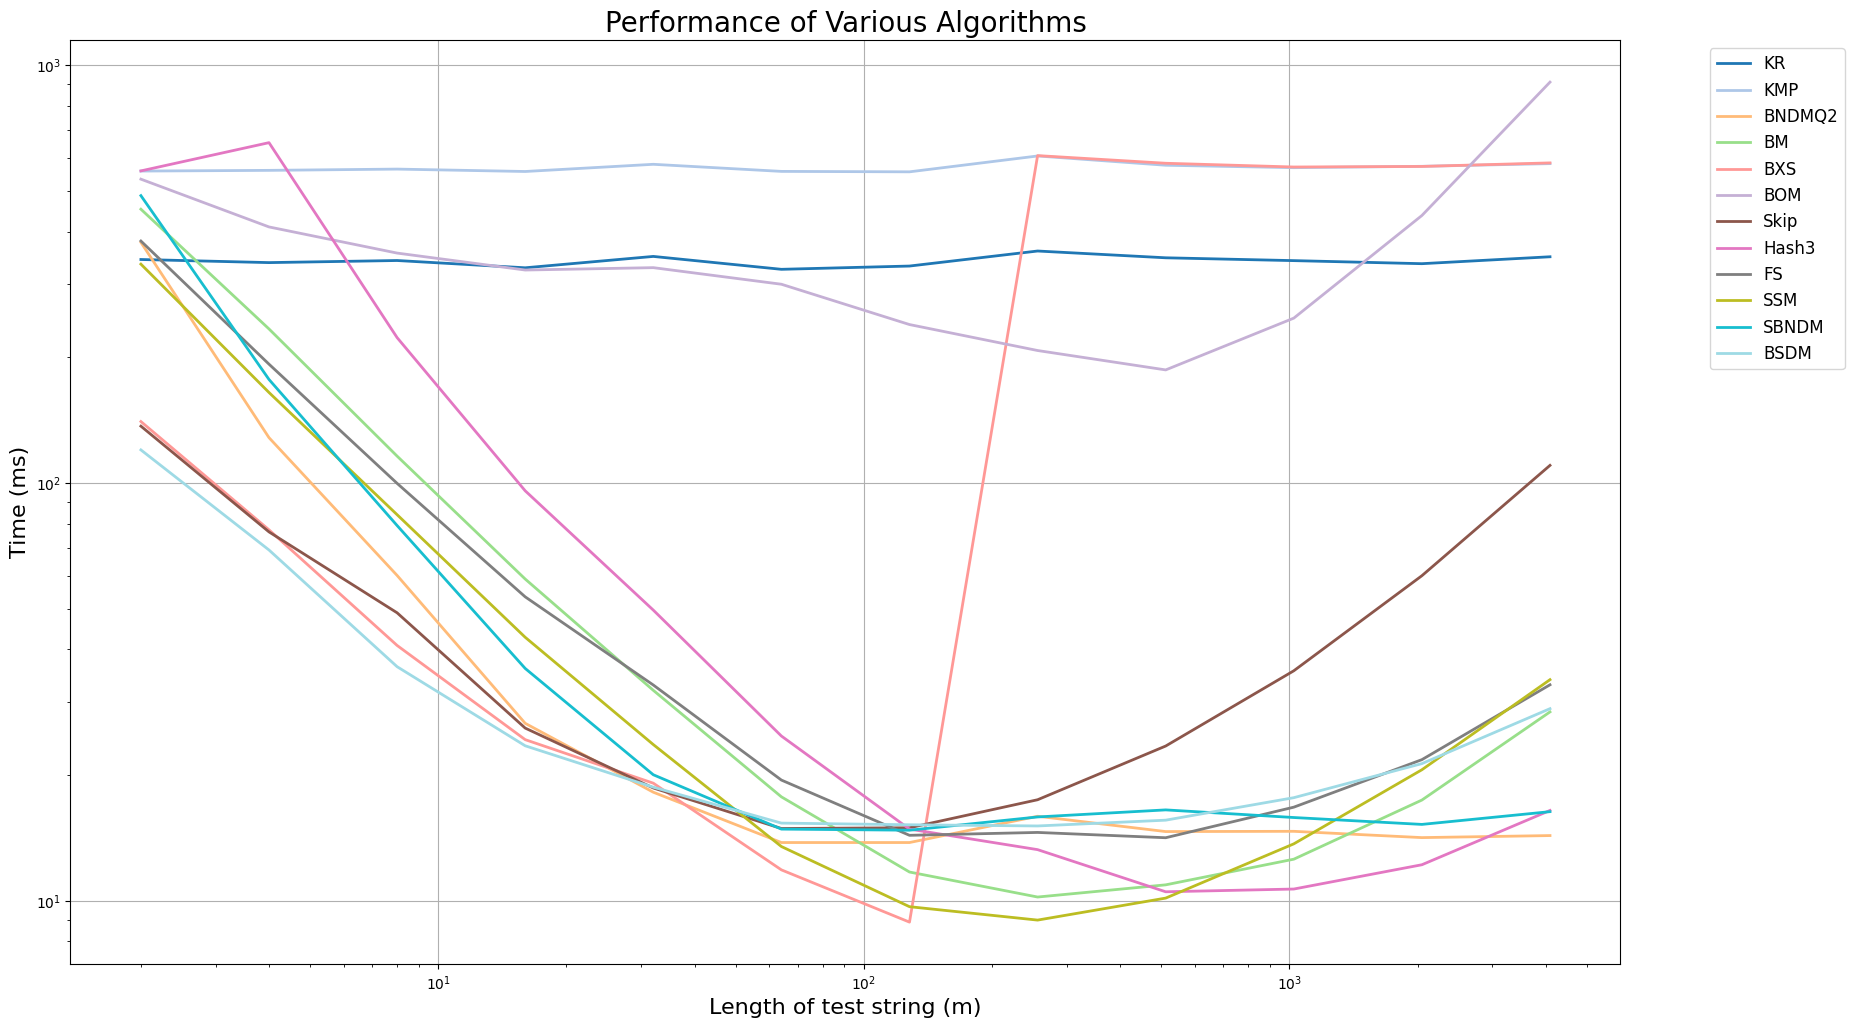
\includegraphics[width=1\textwidth]{images/full_random_graph.png}
						\caption{Залежність часу виконання алгоритмів від довжини патерну}
						\label{fig:full_random_graph}
					\end{figure}

					Перейдемо до загальних результатів роботи алгоритмів за всіма тестами: абсолютних (табл. \ref{table:final_absolute_fullrandom}) та відносних (табл. \ref{table:final_relative_fullrandom}) без врахування довжини патерна m.

					\begin{table}[H]
						\centering
						\scriptsize
						\begin{tabular}{|c|c|c|c|c|c|c|c|c|c|c|c|}
						\hline
						\textbf{KR} & \textbf{KMP} & \textbf{BNDMQ2} & \textbf{BM} & \textbf{BXS} & \textbf{BOM} & \textbf{Skip} & \textbf{Hash3} & \textbf{FS} & \textbf{SSM} & \textbf{SBNDM} & \textbf{BSDM} \\
						\hline
						4084.23 & 6842.45 & 712.01 & 1002.62 & 3242.55 & 4482.62 & 583.66 & 1683.66 & 892.84 & 760.28 & 909.64 & \textbf{397.09} \\
						\hline
						\end{tabular}
						\caption{Сумарні абсолютні результати роботи алгоритмів без врахування $m$ (час у мс)}
						\label{table:final_absolute_fullrandom}
					\end{table}
					
					\begin{table}[H]
						\centering
						\scriptsize
						\begin{tabular}{|c|c|c|c|c|c|c|c|c|c|c|c|c|}
						\hline
						\textbf{KR} & \textbf{KMP} & \textbf{BNDMQ2} & \textbf{BM} & \textbf{BXS} & \textbf{BOM} & \textbf{Skip} & \textbf{Hash3} & \textbf{FS} & \textbf{SSM} & \textbf{SBNDM} & \textbf{BSDM} \\
						\hline
						22.58 & 38.59 & \textbf{0.55} & 1.26 & 21.99 & 29.23 & 2.38 & 2.17 & 1.51 & 1.00 & 0.87 & 0.57 \\
						\hline
						\end{tabular}
						\caption{Середні сумарні відносні результати $\sigma$ без врахування $m$}
						\label{table:final_relative_fullrandom}
					\end{table}
						
					\textbf{Робимо висновки:}

					Три найкращих алгоритмів в загальному випадку за абсолютним показником - \textbf{BSDM, Skip, BNDMQ2}.

					Три найкращих алгоритмів в загальному випадку за відносним показником - \textbf{BNDMQ2, BSDM, SBNDM}.

				\subsection{Порівняння алгоритмів на випадкових патернах із тексту }

				Перейдемо до порівняння алгоритмів на випадкових патернах взятих із тексту.

				Проведемо тестування (табл. \ref{table:lesya}) на українському тексті (Леся Українка <<Лісова пісня>>)
				
				\begin{table}[H]
					\centering
					\scriptsize
					\begin{tabular}{|c|c|c|c|c|c|c|c|c|c|c|c|c|}
					\hline
					\textbf{m} & \textbf{KR} & \textbf{KMP} & \textbf{BNDMQ2} & \textbf{BM} & \textbf{BXS} & \textbf{BOM} & \textbf{Skip} & \textbf{Hash3} & \textbf{FS} & \textbf{SSM} & \textbf{SBNDM} & \textbf{BSDM} \\
					\hline
					2 & 21.46 & 42.67 & 24.25 & 34.30 & 22.26 & 46.36 & 24.92 & 42.41 & 31.15 & 29.54 & 30.49 & \textbf{20.60} \\
					\hline
					4 & 20.99 & 45.64 & \textbf{10.38} & 20.12 & 18.76 & 36.78 & 21.07 & 41.14 & 19.35 & 15.97 & 13.20 & 19.35 \\
					\hline
					8 & 19.62 & 43.86 & \textbf{6.19} & 11.67 & 13.14 & 28.28 & 16.41 & 13.97 & 11.96 & 8.67 & 7.54 & 16.30 \\
					\hline
					16 & 20.03 & 41.32 & \textbf{4.27} & 7.94 & 7.41 & 21.28 & 11.31 & 6.26 & 7.80 & 5.40 & 4.71 & 12.53 \\
					\hline
					32 & 20.08 & 41.37 & \textbf{2.92} & 4.42 & 4.23 & 14.67 & 8.34 & 3.10 & 5.38 & 3.36 & 3.36 & 11.65 \\
					\hline
					64 & 19.75 & 43.88 & 2.97 & 3.41 & 2.74 & 11.07 & 7.65 & \textbf{1.72} & 4.34 & 2.43 & 3.95 & 10.50 \\
					\hline
					128 & 20.21 & 44.75 & 3.55 & 2.32 & 1.87 & 7.82 & 6.70 & \textbf{1.13} & 3.12 & 1.78 & 4.03 & 10.21 \\
					\hline
					256 & 20.19 & 45.15 & 3.26 & 2.10 & 44.55 & 6.15 & 6.26 & \textbf{0.81} & 2.88 & 1.61 & 4.06 & 10.21 \\
					\hline
					512 & 20.44 & 43.59 & 3.07 & 1.81 & 43.31 & 5.57 & 6.89 & \textbf{0.70} & 2.55 & 1.54 & 3.99 & 9.63 \\
					\hline
					1024 & 20.08 & 41.18 & 2.92 & 1.94 & 41.65 & 6.69 & 7.94 & \textbf{0.77} & 2.56 & 1.73 & 3.99 & 9.60 \\
					\hline
					2048 & 20.16 & 41.73 & 3.10 & 2.36 & 42.28 & 10.50 & 10.67 & \textbf{0.96} & 2.87 & 2.39 & 4.04 & 9.88 \\
					\hline
					4096 & 19.75 & 43.42 & 3.06 & 3.90 & 43.28 & 19.16 & 16.53 & \textbf{1.50} & 4.53 & 4.08 & 4.27 & 10.45 \\
					\hline
					\end{tabular}
					\caption{Результати роботи алгоритмів на українському тексті (час у мс)}
					\label{table:lesya}
					\end{table}
				Бачимо, що результати змінились відносно тестування на випадкових патернах на англійському тексті (табл. \ref{table:lotr}).

				Тепер найкращим алгоритм для маленьких $m$ є BNDMQ2, а для великих Hash3.

				Проведемо тестування на випадковій ДНК послідовності (табл. \ref{table:dna_results}).
				\begin{table}[H]
					\centering
					\scriptsize
					\begin{tabular}{|c|c|c|c|c|c|c|c|c|c|c|c|c|}
					\hline
					\textbf{m} & \textbf{KR} & \textbf{KMP} & \textbf{BNDMQ2} & \textbf{BM} & \textbf{BXS} & \textbf{BOM} & \textbf{Skip} & \textbf{Hash3} & \textbf{FS} & \textbf{SSM} & \textbf{SBNDM} & \textbf{BSDM} \\
					\hline
					2 & \textbf{17.91} & 35.83 & 20.40 & 30.04 & 36.79 & 48.05 & 33.49 & 35.87 & 29.82 & 31.38 & 22.88 & 34.89 \\
					\hline
					4 & 13.49 & 36.52 & \textbf{11.89} & 19.75 & 22.75 & 35.10 & 24.53 & 27.20 & 19.04 & 18.03 & 13.29 & 30.04 \\
					\hline
					8 & 13.27 & 36.22 & \textbf{8.41} & 13.72 & 12.42 & 23.79 & 17.83 & 9.57 & 13.54 & 11.47 & 8.81 & 22.98 \\
					\hline
					16 & 13.21 & 35.68 & 5.09 & 11.30 & 6.46 & 15.42 & 14.51 & \textbf{4.50} & 11.27 & 8.13 & 5.15 & 17.66 \\
					\hline
					32 & 12.99 & 37.44 & 2.70 & 9.63 & 3.51 & 9.92 & 12.94 & \textbf{2.43} & 9.86 & 6.40 & 2.74 & 15.32 \\
					\hline
					64 & 12.88 & 36.08 & 2.66 & 8.56 & 2.92 & 6.51 & 11.60 & \textbf{1.57} & 8.63 & 5.01 & 2.71 & 13.78 \\
					\hline
					128 & 12.97 & 36.91 & 2.73 & 7.16 & 2.37 & 4.33 & 10.97 & 1.22 & 7.32 & \textbf{0.89} & 2.80 & 12.83 \\
					\hline
					256 & 13.04 & 36.93 & 2.71 & 6.82 & 37.04 & 3.47 & 11.12 & \textbf{1.04} & 6.93 & \textbf{1.04} & 2.70 & 11.92 \\
					\hline
					512 & 13.96 & 37.29 & 2.71 & 6.34 & 36.49 & 3.44 & 11.50 & \textbf{1.05} & 6.41 & 1.28 & 2.71 & 11.40 \\
					\hline
					1024 & 13.27 & 36.96 & 2.68 & 6.23 & 37.21 & 4.67 & 12.79 & \textbf{1.05} & 6.31 & 1.73 & 2.74 & 11.19 \\
					\hline
					2048 & 13.42 & 38.34 & 2.74 & 5.99 & 38.35 & 8.98 & 17.67 & \textbf{1.36} & 6.24 & 2.83 & 3.07 & 12.11 \\
					\hline
					4096 & 13.37 & 37.97 & 2.74 & 7.77 & 37.80 & 15.99 & 20.99 & \textbf{1.74} & 7.72 & 4.51 & 3.03 & 13.23 \\
					\hline
					\end{tabular}
					\caption{Результати роботи алгоритмів на геномі (час у мс)}
					\label{table:dna_results}
					\end{table}

				Отримуємо результати, схожі на попередні. Алгоритм Hash3 - оптимальний майже для всіх $m>8$. Алгоритм KR вперше показує оптимальний результат для $m=2$.

				Проведемо тестування на великому html файлі (табл. \ref{table:html_random}).

				\begin{table}[H]
					\centering
					\scriptsize
					\begin{tabular}{|c|c|c|c|c|c|c|c|c|c|c|c|c|}
					\hline
					\textbf{m} & \textbf{KR} & \textbf{KMP} & \textbf{BNDMQ2} & \textbf{BM} & \textbf{BXS} & \textbf{BOM} & \textbf{Skip} & \textbf{Hash3} & \textbf{FS} & \textbf{SSM} & \textbf{SBNDM} & \textbf{BSDM} \\
					\hline
					2 & 32.11 & 56.98 & 36.41 & 46.48 & 23.03 & 61.52 & 23.53 & 58.45 & 40.68 & 37.08 & 45.70 & \textbf{20.59} \\
					\hline
					4 & 30.45 & 54.52 & 12.64 & 23.66 & 13.46 & 43.34 & 13.96 & 60.70 & 20.84 & 18.26 & 17.48 & \textbf{12.43} \\
					\hline
					8 & 29.87 & 55.12 & \textbf{6.71} & 13.45 & 11.06 & 36.71 & 11.66 & 20.84 & 11.99 & 10.12 & 8.47 & 11.35 \\
					\hline
					16 & 29.36 & 56.15 & \textbf{3.61} & 7.34 & 7.52 & 26.83 & 9.34 & 9.12 & 6.95 & 5.54 & 4.49 & 10.35 \\
					\hline
					32 & 29.42 & 55.23 & \textbf{2.57} & 4.68 & 4.84 & 21.14 & 6.82 & 4.44 & 4.69 & 3.52 & 2.95 & 9.44 \\
					\hline
					64 & 30.28 & 56.80 & 2.44 & 3.07 & 3.13 & 14.82 & 4.99 & 2.46 & 3.31 & \textbf{2.28} & 4.46 & 8.35 \\
					\hline
					128 & 29.90 & 55.19 & 2.76 & 2.44 & 2.31 & 10.61 & 3.96 & \textbf{1.52} & 2.71 & 1.76 & 4.74 & 9.29 \\
					\hline
					256 & 30.22 & 55.96 & 2.69 & 1.81 & 56.32 & 8.03 & 3.67 & \textbf{1.13} & 2.24 & 1.43 & 4.85 & 7.56 \\
					\hline
					512 & 30.31 & 56.64 & 2.62 & 1.72 & 57.29 & 6.78 & 4.23 & \textbf{0.89} & 2.03 & 1.39 & 4.52 & 7.84 \\
					\hline
					1024 & 30.92 & 57.83 & 2.88 & 1.83 & 57.56 & 8.12 & 6.05 & \textbf{0.96} & 2.24 & 1.91 & 5.25 & 8.14 \\
					\hline
					2048 & 29.77 & 56.97 & 3.03 & 2.35 & 56.96 & 10.55 & 7.99 & \textbf{1.13} & 2.74 & 2.43 & 5.17 & 7.53 \\
					\hline
					4096 & 30.17 & 57.62 & 2.54 & 3.69 & 57.14 & 18.21 & 13.12 & \textbf{1.64} & 4.08 & 4.12 & 4.90 & 8.33 \\
					\hline
					\end{tabular}
					\caption{Результати роботи алгоритмів на html (час у мс)}
					\label{table:html_random}
					\end{table}
				Знову маємо схожі результати, та оптимальні алгоритми.

				Переходимо до сумарних результатів (табл. \ref{table:random_absolute} та табл. \ref{table:random_relative}) по всіх тестах за патернами випадково взятих із текста.
			
				\begin{table}[H]
					\centering
					\scriptsize
					\begin{tabular}{|c|c|c|c|c|c|c|c|c|c|c|c|c|}
					\hline
					\textbf{m} & \textbf{KR} & \textbf{KMP} & \textbf{BNDMQ2} & \textbf{BM} & \textbf{BXS} & \textbf{BOM} & \textbf{Skip} & \textbf{Hash3} & \textbf{FS} & \textbf{SSM} & \textbf{SBNDM} & \textbf{BSDM} \\
					\hline
					2 & 374.92 & 660.26 & 428.31 & 570.82 & 359.54 & 760.31 & 347.00 & 651.42 & 493.74 & 451.27 & 535.91 & \textbf{323.67} \\
					\hline
					4 & 363.12 & 678.12 & \textbf{192.29} & 310.51 & 243.43 & 594.29 & 275.22 & 690.04 & 279.29 & 256.06 & 233.79 & 260.70 \\
					\hline
					8 & 335.65 & 667.56 & \textbf{102.79} & 207.10 & 189.16 & 471.78 & 218.72 & 265.00 & 178.78 & 154.73 & 122.12 & 211.22 \\
					\hline
					16 & 365.14 & 678.24 & \textbf{64.99} & 126.30 & 110.71 & 341.20 & 183.21 & 110.55 & 120.53 & 99.75 & 71.81 & 201.94 \\
					\hline
					32 & 346.49 & 694.28 & \textbf{44.05} & 86.18 & 65.93 & 253.61 & 145.06 & 63.35 & 88.74 & 73.51 & 48.25 & 181.76 \\
					\hline
					64 & 323.95 & 656.93 & 41.14 & 64.28 & 45.93 & 171.26 & 119.71 & \textbf{39.76} & 64.81 & 55.12 & 55.81 & 157.97 \\
					\hline
					128 & 325.15 & 649.50 & 42.94 & 51.08 & 57.76 & 120.45 & 107.05 & \textbf{29.16} & 53.00 & 42.31 & 56.76 & 149.27 \\
					\hline
					256 & 328.25 & 656.58 & 40.98 & 41.47 & 650.56 & 92.13 & 101.41 & \textbf{22.95} & 43.52 & 35.98 & 55.78 & 141.75 \\
					\hline
					512 & 323.57 & 647.19 & 42.59 & 36.10 & 644.54 & 70.22 & 104.69 & \textbf{20.59} & 37.99 & 32.90 & 57.48 & 138.35 \\
					\hline
					1024 & 319.38 & 635.82 & 41.56 & 35.34 & 637.73 & 75.30 & 115.15 & \textbf{19.95} & 38.05 & 33.74 & 56.96 & 135.10 \\
					\hline
					2048 & 323.36 & 641.10 & 42.62 & 37.09 & 639.89 & 110.22 & 143.05 & \textbf{22.93} & 40.62 & 38.94 & 58.02 & 135.27 \\
					\hline
					4096 & 321.62 & 655.37 & 41.94 & 48.57 & 656.43 & 199.86 & 190.99 & \textbf{28.23} & 50.90 & 52.16 & 58.70 & 142.30 \\
					\hline
					\end{tabular}
					\caption{Сумарні абсолютні результати роботи алгоритмів (час у мс)}
					\label{table:random_absolute}
					\end{table}
				
				\begin{table}[H]
					\centering
					\scriptsize
					\begin{tabular}{|c|c|c|c|c|c|c|c|c|c|c|c|c|}
					\hline
					\textbf{m} & \textbf{KR} & \textbf{KMP} & \textbf{BNDMQ2} & \textbf{BM} & \textbf{BXS} & \textbf{BOM} & \textbf{Skip} & \textbf{Hash3} & \textbf{FS} & \textbf{SSM} & \textbf{SBNDM} & \textbf{BSDM} \\
					\hline
					2 & 0.47 & 1.57 & 0.64 & 1.13 & 0.28 & 1.89 & 0.25 & 1.56 & 0.90 & 0.73 & 1.06 & \textbf{0.15} \\
					\hline
					4 & 1.22 & 3.18 & \textbf{0.16} & 0.94 & 0.43 & 2.55 & 0.54 & 3.34 & 0.77 & 0.56 & 0.45 & 0.49 \\
					\hline
					8 & 2.74 & 6.25 & \textbf{0.05} & 1.06 & 0.72 & 3.87 & 1.08 & 1.78 & 0.87 & 0.57 & 0.27 & 1.04 \\
					\hline
					16 & 5.64 & 11.46 & \textbf{0.01} & 1.13 & 0.78 & 5.35 & 1.76 & 1.08 & 1.07 & 0.65 & 0.18 & 1.97 \\
					\hline
					32 & 9.01 & 18.52 & \textbf{0.01} & 1.28 & 0.70 & 6.57 & 2.64 & 0.76 & 1.39 & 0.87 & 0.14 & 3.41 \\
					\hline
					64 & 11.03 & 22.82 & \textbf{0.26} & 1.23 & 0.43 & 5.45 & 2.83 & 0.30 & 1.42 & 0.76 & 0.88 & 4.03 \\
					\hline
					128 & 15.81 & 32.17 & 0.92 & 1.59 & 1.03 & 5.22 & 3.81 & \textbf{0.22} & 1.88 & 0.61 & 1.69 & 5.78 \\
					\hline
					256 & 20.83 & 40.70 & 1.38 & 1.64 & 40.46 & 5.46 & 4.65 & \textbf{0.17} & 1.96 & 0.87 & 2.39 & 6.87 \\
					\hline
					512 & 22.95 & 45.55 & 1.74 & 1.66 & 45.35 & 5.50 & 5.75 & \textbf{0.20} & 2.00 & 1.04 & 2.93 & 7.64 \\
					\hline
					1024 & 22.69 & 45.24 & 1.67 & 1.67 & 45.46 & 6.89 & 6.45 & \textbf{0.13} & 2.03 & 1.19 & 2.99 & 7.23 \\
					\hline
					2048 & 19.73 & 39.60 & 1.37 & 1.64 & 39.60 & 10.98 & 7.81 & \textbf{0.20} & 1.97 & 1.45 & 2.53 & 6.17 \\
					\hline
					4096 & 15.84 & 32.39 & 0.84 & 2.21 & 32.46 & 20.87 & 10.25 & \textbf{0.42} & 2.47 & 2.22 & 1.92 & 5.45 \\
					\hline
					\end{tabular}
					\caption{Середні сумарні відносні результати $\sigma$}
					\label{table:random_relative}
					\end{table}

				Додаємо апроксимовані графіки залежності часу виконання кожного алгоритму (рис. \ref{fig:random_graph}) від довжини патерну.

				\begin{figure}[H]
					\centering
					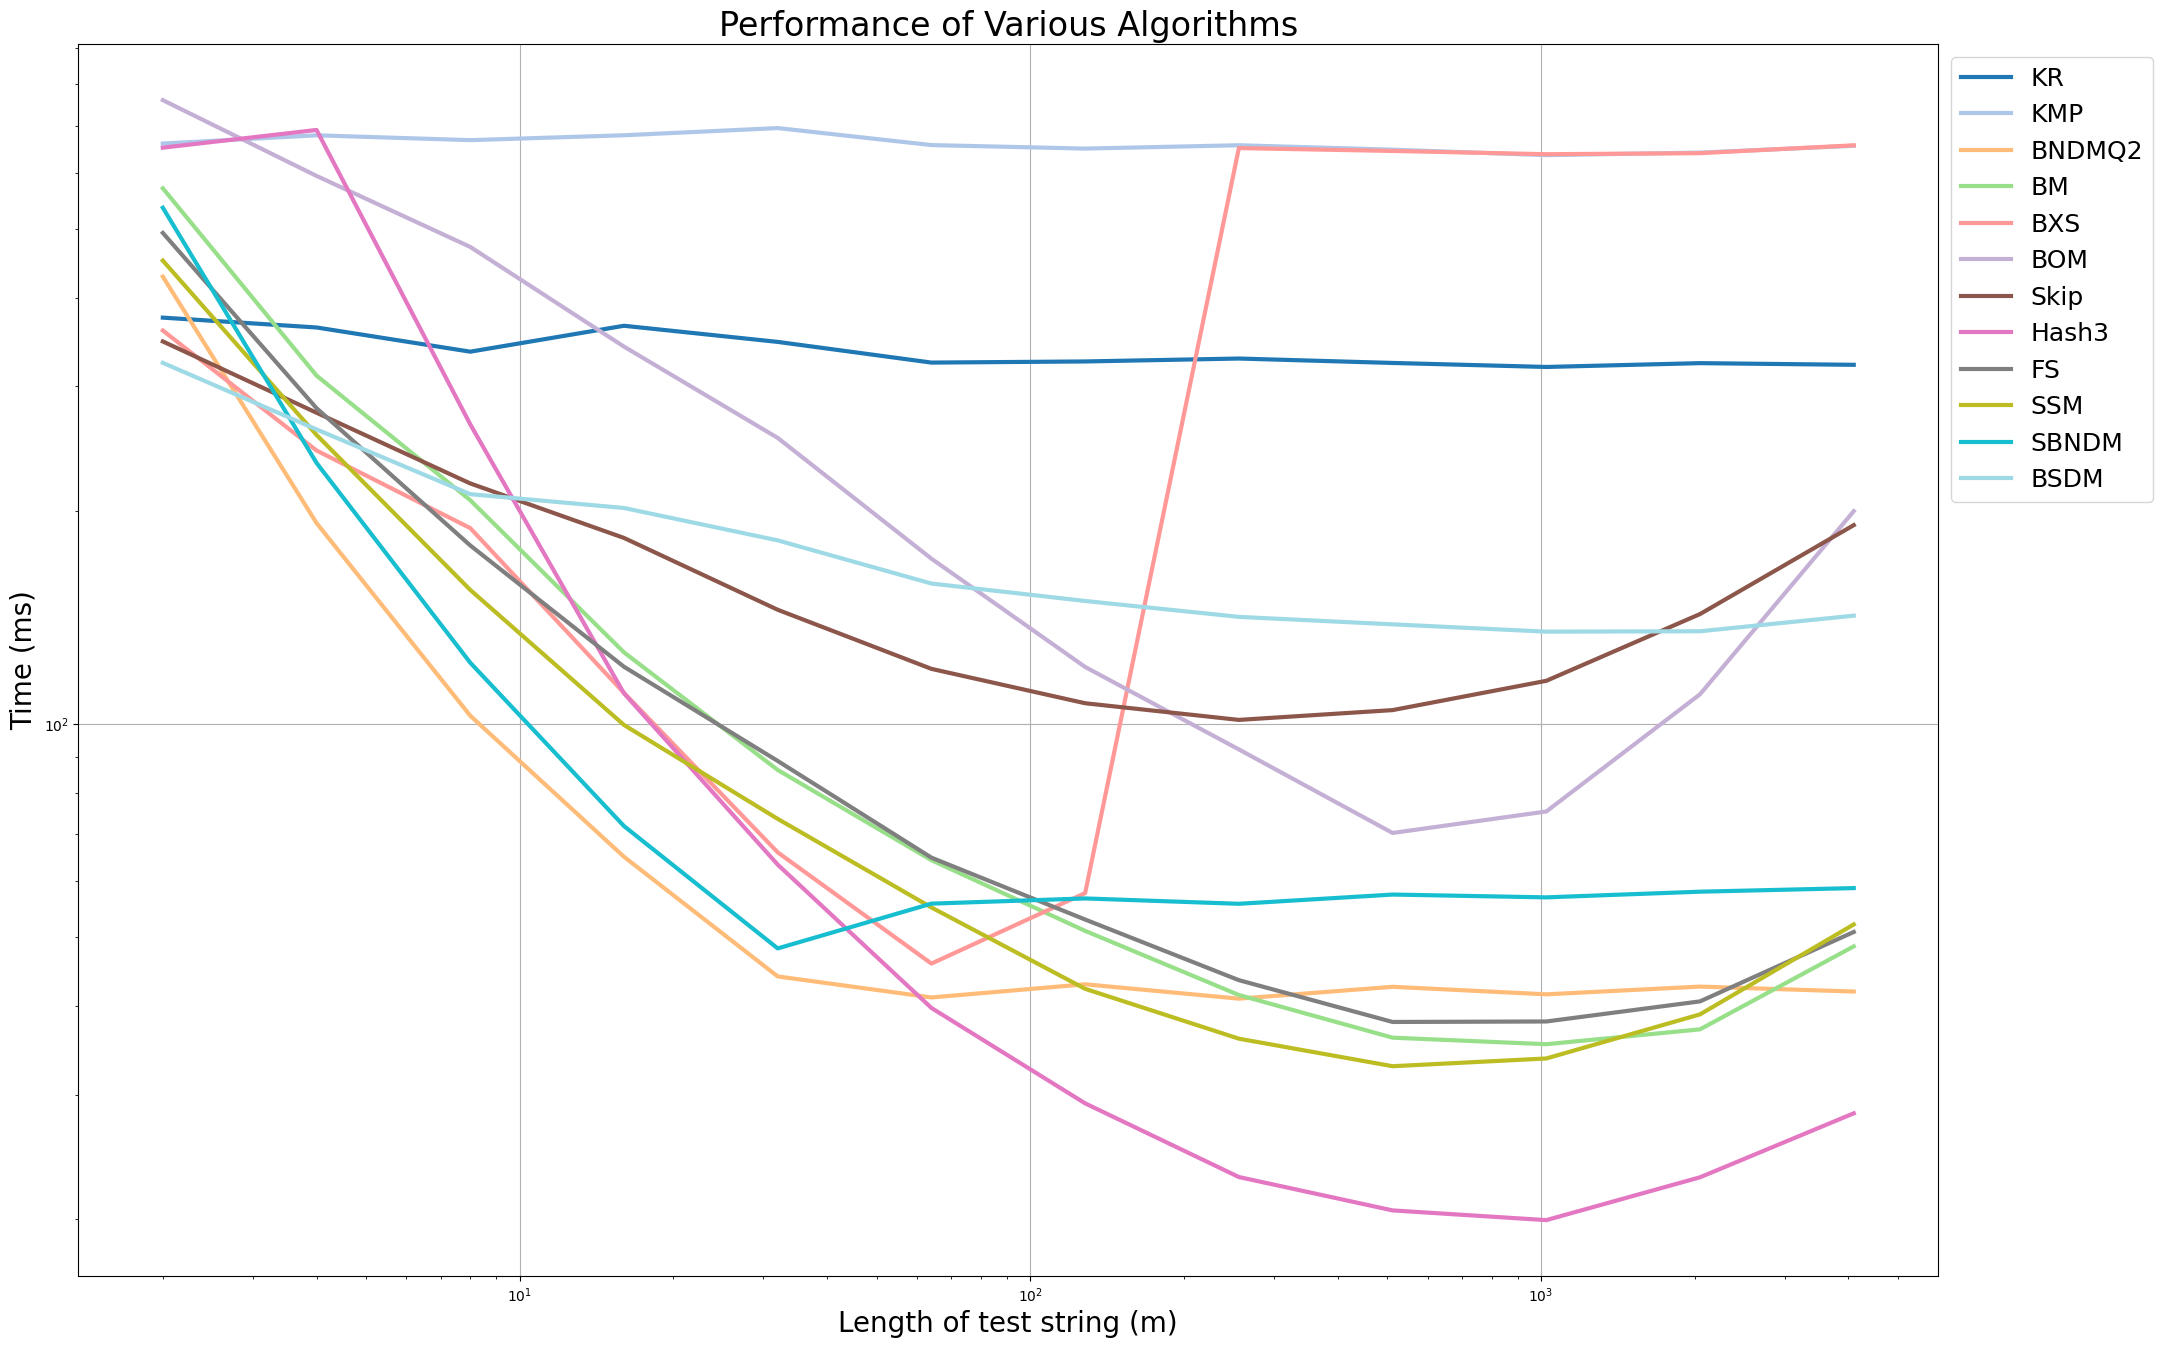
\includegraphics[width=1\textwidth]{images/random_graph.png}
					\caption{Залежність часу виконання алгоритмів від довжини патерну}
					\label{fig:random_graph}
				\end{figure}
				
				Бачимо що оптимальні алгоритми за обома показниками співпадають, окрім $m = 64$.

				Для $m=2$, оптимальним є BSDM. Для інших маленьких $m$ ($2<m<128$) - BNDMQ2. Для великих $m$ - Hash3.
				

				Переходимо до загальних результатів без врахування довжини патерну $m$ (табл. \ref{table:random_final_absolute} та табл. \ref{table:random_final_relative}).
				\begin{table}[H]
					\centering
					\scriptsize
					\begin{tabular}{|c|c|c|c|c|c|c|c|c|c|c|c|c|}
					\hline
					\textbf{KR} & \textbf{KMP} & \textbf{BNDMQ2} & \textbf{BM} & \textbf{BXS} & \textbf{BOM} & \textbf{Skip} & \textbf{Hash3} & \textbf{FS} & \textbf{SSM} & \textbf{SBNDM} & \textbf{BSDM} \\
					\hline
					4050.60 & 7920.95 & \textbf{1126.20} & 1614.84 & 4301.61 & 3260.63 & 2051.26 & 1963.93 & 1489.97 & 1326.47 & 1411.39 & 2179.30 \\
					\hline
					\end{tabular}
					\caption{Сумарні абсолютні результати роботи алгоритмів без врахування m (час у мс)}
					\label{table:random_final_absolute}
				\end{table}

				\begin{table}[H]
					\centering
					\scriptsize
					\begin{tabular}{|c|c|c|c|c|c|c|c|c|c|c|c|c|}
					\hline
					\textbf{KR} & \textbf{KMP} & \textbf{BNDMQ2} & \textbf{BM} & \textbf{BXS} & \textbf{BOM} & \textbf{Skip} & \textbf{Hash3} & \textbf{FS} & \textbf{SSM} & \textbf{SBNDM} & \textbf{BSDM} \\
					\hline
					12.33 & 24.95 & \textbf{0.76} & 1.43 & 17.31 & 6.72 & 3.98 & 0.85 & 1.56 & 0.96 & 1.45 & 4.19 \\
					\hline
					\end{tabular}
					\caption{Середні сумарні відносні результати $\sigma$ без врахування $m$}
					\label{table:random_final_relative}
				\end{table}
				\textbf{Робимо висновки:}

				Три найкращих алгоритмів в загальному випадку за абсолютним показником - \textbf{BNDMQ2, SSM, SBNDM}.

				Три найкращих алгоритмів в загальному випадку за відносним показником - \textbf{BNDMQ2, Hash3, SSM}.

				\subsection{Порівняння алгоритмів на повторюваних патернах із тексту}

				В цьому підрозділі порівняємо алгоритми на патернах, що часто зустрічаються в тексті.
				
				Зазначимо, що в цьому підрозділі не будемо порівнювати результати в залежності від $m$, ажде всі обрані часто повторювані слова у текстах будуть невеликої довжини ($2<=m<=10$).

				Проведемо тестування на англійському тексті (табл. \ref{table:uniqueEnglish}). Патерни беруться, як найбільш повторювані слова англійської мови.
				\begin{table}[H]
					\centering
					\scriptsize
					\begin{tabular}{|c|c|c|c|c|c|c|c|c|c|c|c|c|}
					\hline
					\textbf{KR} & \textbf{KMP} & \textbf{BNDMQ2} & \textbf{BM} & \textbf{BXS} & \textbf{BOM} & \textbf{Skip} & \textbf{Hash3} & \textbf{FS} & \textbf{SSM} & \textbf{SBNDM} & \textbf{BSDM} \\
					\hline
					131.42 & 246.49 & \textbf{36.25} & 75.40 & 52.82 & 164.27 & 59.46 & 171.63 & 65.73 & 60.62 & 49.05 & 57.00 \\
					\hline
					\end{tabular}
					\caption{Результати роботи алгоритмів на англ. тексті (час у мс)}
					\label{table:uniqueEnglish}
				\end{table}

				Проведемо тестування на українському тексті (табл. \ref{table:uniqueUkrainian}). Патерни беруться, як найбільш повторювані слова української мови.
				\begin{table}[H]
					\centering
					\scriptsize
					\begin{tabular}{|c|c|c|c|c|c|c|c|c|c|c|c|c|}
					\hline
					\textbf{KR} & \textbf{KMP} & \textbf{BNDMQ2} & \textbf{BM} & \textbf{BXS} & \textbf{BOM} & \textbf{Skip} & \textbf{Hash3} & \textbf{FS} & \textbf{SSM} & \textbf{SBNDM} & \textbf{BSDM} \\
					\hline
					19.40 & 49.01 & \textbf{5.60} & 9.62 & 12.07 & 25.41 & 18.00 & 14.11 & 8.25 & 7.47 & 6.72 & 15.73 \\
					\hline
					\end{tabular}
					\caption{Результати роботи алгоритмів на укр. тексті (час у мс)}
					\label{table:uniqueUkrainian}
				\end{table}
				
				Проведемо тестування на довгому тексті мовою програмування $c$ (табл. \ref{table:uniqueC}). Патерни беруться, як ключові слова мови програмування $c$.
				\begin{table}[H]
					\centering
					\scriptsize
					\begin{tabular}{|c|c|c|c|c|c|c|c|c|c|c|c|c|}
					\hline
					\textbf{KR} & \textbf{KMP} & \textbf{BNDMQ2} & \textbf{BM} & \textbf{BXS} & \textbf{BOM} & \textbf{Skip} & \textbf{Hash3} & \textbf{FS} & \textbf{SSM} & \textbf{SBNDM} & \textbf{BSDM} \\
					\hline
					50.25 & 84.66 & 18.01 & 31.36 & 15.92 & 60.09 & 15.93 & 64.89 & 26.86 & 23.96 & 24.71 & \textbf{14.69} \\
					\hline
					\end{tabular}
					\caption{Результати роботи алгоритмів на тексті мовою програмування $c$ (час у мс)}
					\label{table:uniqueC}
				\end{table}

				Проведемо тестування на великому html файлі (табл. \ref{table:uniqueHtml}). Патерни обрані, як ключові слова мови HTML.
				\begin{table}[H]
					\centering
					\scriptsize
					\begin{tabular}{|c|c|c|c|c|c|c|c|c|c|c|c|c|}
					\hline
					\textbf{KR} & \textbf{KMP} & \textbf{BNDMQ2} & \textbf{BM} & \textbf{BXS} & \textbf{BOM} & \textbf{Skip} & \textbf{Hash3} & \textbf{FS} & \textbf{SSM} & \textbf{SBNDM} & \textbf{BSDM} \\
					\hline
					32.05 & 52.25 & 12.10 & 20.12 & \textbf{9.37} & 37.92 & 9.79 & 37.54 & 17.28 & 16.81 & 16.69 & 9.81 \\
					\hline
					\end{tabular}
					\caption{Результати роботи алгоритмів на великому html файлі (час у мс)}
					\label{table:uniqueHtml}
				\end{table}

				Проводимо тестування на json базі даних (табл. \ref{table:uniqueJson}). Патерни обрані, як найбільш повторювані поля та значення бази.
				\begin{table}[H]
					\centering
					\scriptsize
					\begin{tabular}{|c|c|c|c|c|c|c|c|c|c|c|c|c|}
					\hline
					\textbf{KR} & \textbf{KMP} & \textbf{BNDMQ2} & \textbf{BM} & \textbf{BXS} & \textbf{BOM} & \textbf{Skip} & \textbf{Hash3} & \textbf{FS} & \textbf{SSM} & \textbf{SBNDM} & \textbf{BSDM} \\
					\hline
					38.88 & 64.95 & \textbf{10.08} & 16.11 & 11.65 & 42.60 & 10.75 & 27.88 & 14.98 & 13.08 & 12.38 & 10.84 \\
					\hline
					\end{tabular}
					\caption{Результати роботи алгоритмів на json файлі (час у мс)}
					\label{table:uniqueJson}
				\end{table}
					
				Переходимо до загальних абсолютних і відносних результатів, (табл. \ref{table:uniqueAbsolute} та табл. \ref{table:uniqueRelative}) за всіма тестами.

				\begin{table}[H]
					\centering
					\scriptsize
					\begin{tabular}{|c|c|c|c|c|c|c|c|c|c|c|c|c|}
					\hline
					\textbf{KR} & \textbf{KMP} & \textbf{BNDMQ2} & \textbf{BM} & \textbf{BXS} & \textbf{BOM} & \textbf{Skip} & \textbf{Hash3} & \textbf{FS} & \textbf{SSM} & \textbf{SBNDM} & \textbf{BSDM} \\
					\hline
					285.34 & 532.20 & \textbf{91.69} & 169.28 & 119.03 & 357.43 & 134.37 & 334.03 & 149.65 & 136.82 & 120.15 & 135.43 \\
					\hline
					\end{tabular}
					\caption{Сумарні абсолютні результати роботи алгоритмів (час у мс)}
					\label{table:uniqueAbsolute}
				\end{table}
				
				\begin{table}[H]
					\centering
					\scriptsize
					\begin{tabular}{|c|c|c|c|c|c|c|c|c|c|c|c|c|}
					\hline
					\textbf{KR} & \textbf{KMP} & \textbf{BNDMQ2} & \textbf{BM} & \textbf{BXS} & \textbf{BOM} & \textbf{Skip} & \textbf{Hash3} & \textbf{FS} & \textbf{SSM} & \textbf{SBNDM} & \textbf{BSDM} \\
					\hline
					2.20 & 5.16 & \textbf{0.09} & 0.90 & 0.44 & 3.04 & 0.69 & 2.38 & 0.69 & 0.55 & 0.39 & 0.72 \\
					\hline
					\end{tabular}
					\caption{Середні сумарні відносні результати $\sigma$}
					\label{table:uniqueRelative}
				\end{table}

				\textbf{Робимо висновки:}

				Три найкращих алгоритми в загальному випадку за абсолютним показником - \textbf{BNDMQ2, BXS, SBNDM}.

				Три найкращих алгоритми в загальному випадку за відносним показником - \textbf{BNDMQ2, SBNDM, BXS}.
					
			\subsection{Підведення підсумків та порівнювання за розміром алфавіту}

			\textbf{За результатами попередніх підрозділів сформуємо таблицю отриманих результатів:}
			
			таблицю найоптимальніших алгоритмів серед заданих (підрозділ \ref{section:algorithms_set}) за типом патерну та за типом оцінки результату (табл. \ref{table:all}).

			\begin{table}[H]
				\centering
				\footnotesize
				\begin{tabular}{|c|c|c|}
				\hline 
				& За абсолютним показником & За відносним показником \\
				\hline 
				Випадкові патерни  & \textbf{BSDM}, Skip, BNDMQ2 & \textbf{BNDMQ2}, BSDM, SBNDM \\
				\hline
				Випадкові патерни, взяті з тексту & \textbf{BNDMQ2}, SSM, SBNDM & \textbf{BNDMQ2}, Hash3, SSM \\
				\hline
				Патерни, що часто зустрічаються & \textbf{BNDMQ2}, BXS, SBNDM & \textbf{BNDMQ2}, SBNDM, BXS \\
				\hline
				\end{tabular}
				\caption{Узагальнююча таблиця найкращих алгоритмів, за типом патернів та за типом результатів}
				\label {table:all}
			\end{table}

			Можемо зробити висновок, що найоптимальнішим алгоритмом з нашого набору є \textbf{BNDMQ2}. А другі і треті місця за оптимальністю відрізняються в залежності від патерну та типу оцінки. Бачимо серед найоптимальніших алгоритмів представників різних класів, отже можемо зробити висновок, що різні класи алгоритмів можуть бути корисними в залежності від умов задачі.
			
			Також було проведено порівняння часу виконання алгоритмів (рис. \ref{fig:sigma_results}) за розміром алфавіту та розміром патерна (на випадкових текстах з алфавітом заданого розміру). Колір відповідної комірки позначає, оптимальний алгоритм для заданого $\Sigma$ та $m$.

			\begin{figure}[H]
				\centering
				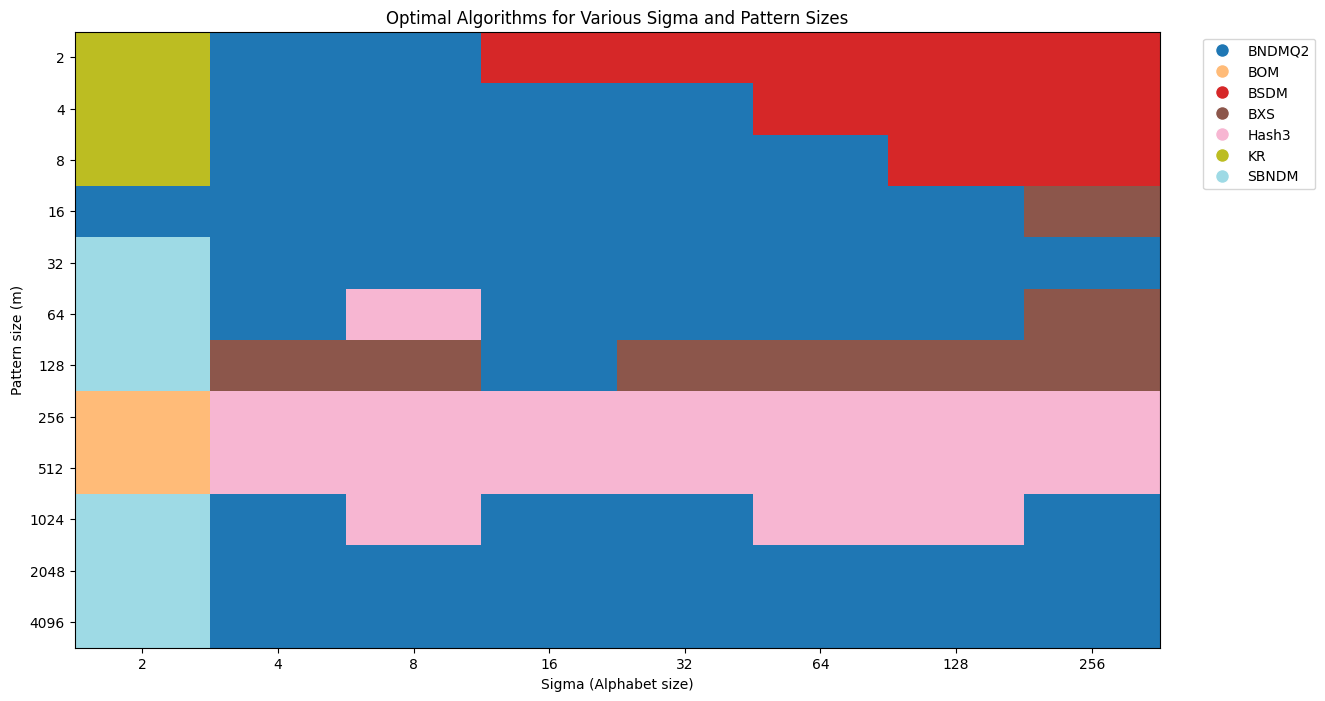
\includegraphics[width=1\textwidth]{images/sigma_results.png}
				\caption{Heatmap найкращих алгоритмів, за розміром алфавіту та за розміром патерна}
				\label{fig:sigma_results}
			\end{figure}
				% Висновки

			Бачимо, що для $m<128$ та $m>512$, для більшості алфавітів найоптимальнішим є BNDMQ2. Для маленьких патернів та великих алфавітів - оптимальний BSDM.
			Для $m=128$ найкращим алгоритмом є BXS. Та для $m\in \{256,512\}$ - Hash3.
	\newpage
    \section*{Висновки}
	\addcontentsline{toc}{section}{Висновки}
	\textbf{Отже у даній роботі було:}
	\begin{itemize}
		\item Виконано огляд та аналіз існуючих алгоритмів патерн-метчингу, наведено їх класифікацію та були описані деякі їх класичні представники.
		\item Розроблено методику порівняння ефективності алгоритмів патерн-метчингу.
		\item Виконано порівняння ефективності набору алгоритмів за допомогою розробленої методики на практиці.
		\item Продемонстровано та проаналізовано результати порівняння алгоритмів.
	\end{itemize}

	\textbf{Можливі розвинення та інші дослідження заданої тематики:}
	\begin{itemize}
		\item Порівняння ефективності алгоритмів патерн-метчингу в залежності від їх класу.
		\item Порівняння ефективності <<офлайн>> патерн-метчинг алгоритмів.
		\item Порівняння ефективності алгоритмів на <<найгірших>> патернах. Знайти найефективніший алгоритм, при найгірших вхідних даних для кожного алгоритму.
		\item Порівняння ефективності <<approximate string searching>> алгоритмів.
		\item Розробити повноцінний застосунок, що буде знаходити оптимальний алгоритм, за заданими параметрами задачі користувача.
		\item Остання знайдена мною оглядова робота за сучасними алгоритмами патерн-метчингу датована 2019 роком \cite{2019survey}. Отже цікавим напрямом є аналіз та оцінка ефективності алгоритмів патерн-метчингу створених в 2020-2024 роках.
	\end{itemize}

    \newpage
    
    % Список літератури
    \begin{thebibliography}{9}
        \addcontentsline{toc}{section}{Література} % Добавление списка литературы в оглавление
		\bibitem{dna}
		Alsmadi, I., \& Nuser, M. (2012). String matching evaluation methods for DNA comparison. International Journal of Advanced Science and Technology, 47(1), 13-32.
		\bibitem{morris-pratt}
		J. H. Morris, Jr and V. R. Pratt. A linear pattern-matching algorithm. Report 40, University of California, Berkeley, 1970.
		\bibitem{smart}
		Faro, S., \& Lecroq, T., Borzi, S., Di Mauro, S.,\& Maggio, A. (2016, August). The String Matching Algorithms Research Tool. In Stringology (pp. 99-111).
		\bibitem{exact}
		Faro, S., \& Lecroq, T. (2013). The exact online string matching problem: A review of the most recent results. ACM Computing Surveys (CSUR), 45(2), 1-42.
		\bibitem{bm}
		R. S. Boyer and J. S. Moore. A fast string searching algorithm. Commun.
ACM, 20(10):762–772, 1977.
		\bibitem{experiment}
		Faro, S., \& Lecroq, T. (2010). The exact string matching problem:
		
		a comprehensive experimental evaluation. arXiv preprint arXiv:1012.2547.

		\bibitem{2019survey}
		Hakak, S. I., Kamsin, A., Shivakumara, P., Gilkar, G. A., Khan, W. Z., \& Imran, M. (2019). Exact string matching algorithms: survey, issues, and future research directions. IEEE access, 7, 69614-69637.
		\bibitem{FDM}
		M. Crochemore and W. Rytter. Text algorithms. Oxford University Press,
1994.
		\bibitem{survey2014}
		Al-Khamaiseh, K., \& ALShagarin, S. (2014). A survey of string matching algorithms. Int. J. Eng. Res. Appl, 4(7), 144-156.

    \end{thebibliography}
    
	\newpage

	\section*{Додаток А}
	\addcontentsline{toc}{section}{Додаток А}

	Посилання на вихідний код алгоритмів, основної програми, що виконувала тестування, та тести з отриманими результатами:

	\small{\url{https://github.com/DeDTihoN/StringPatternAlgorithmsTesting}}
\end{document}